\chapter{\texorpdfstring{DATA ANALYSIS AND FINDINGS}{}} %upper case only

In this chapter, I present the findings of the analysis about identity negotiations that emerged from the lived experiences of first, one and a half and second-generation Pakistani families in the US. Themes are introduced through representative found poems, accompanied by analytic interpretation that illustrates how identity meanings emerge from retrospective storytelling and travel across CTI five layers.

I collected the stories using individual episodic in-depth narrative interviews. I used the theoretical lens of CNSM’s retrospective storytelling heuristic and CTI to interpret these interviews. I paid particular attention to the material frame of CTI based on the fact that it is recently added to the layers of CTI and is also the most visible and tangible layer that can be seen and influenced in/by physical space and time, identity gaps, and negotiation. The purpose of this study was to examine the ways in which the first generation of Pakistani immigrants navigated their identities and guided the identity development and negotiation process of their children in the US. I was interested in how immigrant family members across the generations tell family stories of the past using retrospective storytelling as a medium to communicate the process of identity development through the challenges of shifting identities within familial and public contexts. 

Building on CTI’s assertion that identity is communication and vice versa, this study positions retrospective storytelling as the processing channel through which identity layers are not only expressed but brought into interaction with one another. When participants recount past experiences, they do more than describe events; they actively reconstruct meanings of self (personal), demonstrate identity in communication (enacted), position themselves in relation to others (relational), draw upon shared cultural narratives (communal), and anchor these meanings within lived environments and constraints (material). Thus, retrospective storytelling operates as a dynamic site of identity work where these layers converge, often revealing tensions, alignments, and transformations. This process is especially salient in intergenerational immigrant contexts, where stories become vehicles for transmitting values, negotiating belonging, and shaping future generations’ identity. I also examined the role of retrospective storytelling in sharing intergenerational values and lived experiences, and how such practices shape identity negotiation within Pakistani families living in the US. 

\section{Analysis Approach}

Four research questions guided the thematic analysis by addressing the epistemological questions concerning the integration of CTI and CNSM theories as well as enhancing “understanding” the phenomena of” (Faulkner \& Atkinson, 2024, p.79) shifting identities and identity negotiation. I used poetic inquiry as an analytic tool to conduct a thematic analysis. Through poetic inquiry, I created poetic transcripts and found poems, drawn directly from participants’ original words, rhythms, and emotions. Participants’ stories were not treated as data alone; rather, poetic transcripts were created to preserve the affective, relational, and embodied qualities of the stories shared by interviewees. These poetic transcripts functioned simultaneously as a mode of analysis and as the presentation of the findings (Faulkner, 2023, 2019b). 
The first two research questions explored the employment of retrospective storytelling (the process and the content) by Pakistani American families to make sense of their shifting identities within the household and in public. The third and fourth questions focused on the projection of the material frame of CTI in the identity negotiation process between first-generation and one-and-a-half and second-generation immigrants. To reiterate, the research questions (RQ) of this study are as follows.

\subsection{Research Questions}

\begin{enumerate}
    \item How do Pakistani American families employ retrospective storytelling and narrative sharing to make sense of their identities within the household and in public?
    \item How does the content and process of storytelling (individual, relational, and intergenerational meaning-making of values and beliefs) reflect in Pakistani American immigrants’ material frame of identity?
    \item How does the five frames of CTI project in the process of identity negotiation between first-generation and one-and-a-half and second-generation immigrants?
    \item Are there gaps in identity for Pakistani immigrants? If so, what are the gaps and how do these gaps influence identity negotiation?
\end{enumerate}

\section{Presentation of Poetic Themes}

The themes that emerged from the poetic analysis are presented as poetic transcripts and poems that honored the participants’ experiences in their own voices and brought the emotional and embodied layers of their identity to the forefront. Although the themes are organized in relation to specific research questions, several themes speak to multiple questions simultaneously. This overlap reflects the nuanced and intersecting nature of the participants’ lived experiences, wherein a single theme often addresses multiple dimensions of identity at once. Nevertheless, all themes directly emerged from participants’ accounts and collectively addressed the guiding research questions through the analytical lenses of CTI and CNSM theory. Each theme captures a distinct dimension of how identity is communicated, contested, and lived within Pakistani migrant families.

\subsection{Making Sense of Shifting Identities through Retrospective Storytelling}

Poetic transcripts and found poems preserved the affective and relational textures of participants’ stories, allowing the layered meanings of their inherited and lived experiences to come to the surface. Data revealed family narratives as complex, nonlinear archives of conditioning and expectations. These narratives reflected a strong presence of emotional codependence, gendered familial responsibility, guilt, fear, obligation, faith, and longing for home. 

Within these stories, identity emerged as a dynamic process of verbal and nonverbal communication shaped by the environments, territorial locations, as well as the physical conditions through which families lived their daily lives. 

The practice of retrospective storytelling emerged as an everyday, habitual and emotionally saturated practice through which families interpreted past events, constructed meanings in the present time, and negotiated the challenges of shifting identities. Parents, mothers in particular, used stories to share their silent journeys of sacrifices and migration as well as to establish familial expectations and values, and regulate boundaries between Pakistani and American cultural territories.

The following themes present the content and process of retrospective storytelling as participants made sense of changing relational and communal layers of identities.

\subsection{Theme 1: Migration, Visa Pathways, and Life-Course Outcomes}

The following set of poetic transcripts and poems reflects the first-generation migrants making sense of migration and shifting identities in the US. For many first-generation Pakistani women, retrospective storytelling becomes a central interpretive tool allowing them to frame migration as kismet (fate) or something meant to be. In contrast, many male participants framed migration not as ambition, but as unplanned transition driven by circumstances or global sociopolitical and economic conditions. Another factor that significantly informed migration decisions was gender and marital status. While men were mostly allowed travel to the US for higher education or pursuit of professional excellence, most Pakistani women were only sent to the US after getting married as dependents of their spouses. Further, the gender of their children influenced the challenges they encountered, the strategies they employed, and the ways the identity expectations were negotiated across specific social, cultural, and temporal contexts.

The following poem, titled Kismet meaning “fated to be” or guided by God’s will reflects WJ’s narrative of migration, gendered decision-making, and identity negotiation. Dr.~WJ, who worked as a dentist in Karachi, Pakistan, moved to the United States after marriage and is now a homemaker, mother of three young daughters, and philanthropist. She is married to a Pakistani physician and currently resides in Sylvania, Ohio. 

\begin{FoundPoem}
    I never dreamed  
    (moving abroad)

    Lugon ko hota na
    you know,
    some people carry that dream
    in their minds

    I never wanted it,
    and neither did my parents.

    My parents had a green card,
    yet they decided
    to stay back in Pakistan.

    We are four sisters.

    My parents decided
    not to settle in the US
    they did not like the environment
    for raising girls.

    But we believe in kismet.
    We believe in fate.
    I got married.
    My husband was doing his residency
    in the US.
    I moved. 
\end{FoundPoem}

In her account, WJ reflects on her parents’ decision to not settle in the US despite having the opportunity to do so, citing concerns about raising four daughters in what they perceived as an unsuitable environment for girls. 

WJ described herself as an accomplished dentist who had to forgo her professional career following her marriage. After relocating to the US, she passed all three required board examinations within a few months. However, when the prospect of moving to another city for residency arose, she was advised by her parents and parents-in-law not to pursue further studies if doing so required living separately from her husband. 


\begin{FoundPoem}
    
    I was doing my FCPS in Pakistan, a fellowship 		training in
    maxillofacial surgery. But 		I came here, there is a very long pathway
    for dentistry, unlike the medicine. 
     My husband,    took the exams,    applied for the residency
        immediately get into it. 	
        For the	                     international dentists,                       very selected
    programs, 		  only in the major cities.
        In three months, I took all my board exams;   passed all of them.
  
    From my parents’ and	 my parents-in-law	
    told me to stay wherever he(husband) goes for his fellowship. 
    Don’t move away from your husband, they said.

I was tempted. I was bored. There was nothing for me. Nobody knew me.
        From  
    Dr. WJ in Karachi to now I am identified as Dr. Zaidi’s wife 
    And I felt 			   a big gap,  
    But then, being a very traditional wife, newlywed
    Thought, I should just stay with my husband 
    wherever he’s doing his residency. 
    Unfortunately, he moved cities, but they did not have 
    any dental programs for me or dental schools. 
    They were in New York or Chicago, major cities. I decided not to stay away for
    three years of a dental program to do my residency, So I stayed back, just
    hoping for the luck 
    We ended up in Toledo. Toledo does not offer any. 
    The closest would be Detroit. 
    But now, I’m so invested with my family, my daughters 
    But
    I still have that void in my life. 
    Alhamdulillah,  				I’m so blessed,
        I have everything. 		 I’ve been very busy with other
        philanthropic work in the US and back in Pakistan.

\end{FoundPoem}

After becoming a parent, WJ was expected to prioritize children’s needs until the daughters were fully settled in their careers. This kind of expectation creates an ambivalent and, at times, confusing environment for children, particularly, daughters who observe their mother occupying a primarily domestic and supportive role while simultaneously receiving strong encouragement to pursue higher education, professional success, and individual independence. As daughters are socialized to develop autonomous professional identities, they are also exposed to a contrasting relational model in which maternal self-sacrifice and emotional labor are normalized and rarely questioned. When these daughters later transition into the roles of wife and mother, they may experience tension and uncertainty as they attempt to reconcile these competing identity scripts: whether to emulate their mothers’ caregiving roles or to enact the career-oriented identities they were encouraged to cultivate.

Maheen accompanied her parents to the US at age 12 in 2009, following family sponsored immigration through her phopho (paternal aunt) to Chicago. She saw her parents with college degrees working odd jobs in the US. Maheen, now 28-years old and working full time as a tax consultant for a company in Chicago, sees herself as a working mother. She currently lives in Chicago with her husband, a 3-year-old son, a 3-month-old baby boy, and a widowed mother-in-law. She shared that when she is at work all she is thinking of is how her two baby boys are doing and once home what chores need to be done. These tasks include bathing the boys and preparing meals for the family. While Maheen reflected on her experiences as she transitioned from being a daughter to a wife, daughter-in-law, and a mother, she shared feeling like she was juggling too many balls at once.

\begin{FoundPoem}
In Pakistani culture,
a daughter-in-law becomes
everyone’s maid.

No matter how good the husband is,
if you live in a joint family,
or with the in-laws,
you become
a maid for all of them.

That’s how my mom was.

I grew up watching her like that.
No
I never thought of her as a maid.
I thought,
this is what a mother does.

I grew up watching her do everything. 

Thought, this is what she needs to do,		
She’s the mom
All moms
 do the same 
until I got married 
        became a mother
glad
didn’t gave up my career, 
did not follow the same path like her

But
I could not say no
grew up saying yes
seeing my mom 
I started doing the same
Like my mom do it
Until
mom reminded me 
Don’t 
Later
expectations grow higher
and can’t be met
Relationships get harder 

Dads are different
for their daughters
than for their wives.

Yes.
There’s a constant conversation
between my mom and dad.

When it happens to your daughter,
you react like this.
When it happened to me,
you never said anything.

\end{FoundPoem}

Maheen’s narrative highlights the gendered precarity of women’s labor within both Pakistani and migrant family contexts, while also revealing how intergenerational expectations are reproduced and negotiated through marriage, caregiving, and everyday relational roles. A key contextual factor is that Maheen’s marriage was arranged transnationally: she traveled to Pakistan for the wedding, and her husband later emigrated to the United States on a spousal visa. This transnational pathway produced an additional generational and adjustment gap within the couple’s early marital life, shaped by uneven familiarity with the US social system, settlement pressures, and shifting household responsibilities.

This intergenerational contradiction becomes further visible when considered alongside Maheen’s narrative. Similar to WJ’s experience, where maternal self-sacrifice was normalized even as daughters were encouraged to pursue professional success, Maheen’s story revealed how gendered expectations operate unevenly across relational roles. While daughters are urged to cultivate autonomy and career-oriented identities, the relational model they often witness continues to valorize women’s endurance, accommodation, and caregiving as taken-for-granted obligations. This contradiction becomes especially visible in Maheen’s observation of her father’s protective scrutiny of her marriage: questioning her husband’s absence and attentiveness in ways he did not enact on behalf of his wife in earlier years. Together, these narratives demonstrate how migrant families simultaneously promote daughters’ independence while sustaining relational scripts that reproduce gendered responsibility and emotional labor within marriage and family life.

As these daughters transition into wifehood and motherhood, they are left to negotiate competing identity scripts: whether to reproduce maternal patterns of self-effacing care or to enact the career-oriented identities they were urged to develop. 

Building this intergenerational tension, the next theme examines how some parents make deliberate migration decisions to disrupt inherited gendered constraints and create the conditions under which their children’s identities develop.

\subsection{Theme 2: Gendered Migration and Parental Decision-Making}

Parents’ narratives revealed contrasting orientations toward migration and settlement that were deeply intertwined with the shifting identities of both parents and children across households and public contexts. While some parents expressed concerns about their daughters’ safety and viewed the United States as an unsuitable environment for raising children, particularly girls, others made intentional decisions to remain and settle in the US to secure greater autonomy, visibility, and opportunity for their daughters. These decisions shaped how parents understood their own roles and responsibilities, as well as how children learned to navigate identity expectations at home and in broader social spaces.

Wali, a 45-year-old Pakistani man, migrated to the US with his wife as newlyweds in the early 2000s to pursue a Ph.D., with no initial intention of permanent settlement. Now a father of three daughters and residing in New Jersey, he described how his plans shifted as his family grew. He ultimately decided to remain in the US, framing this choice as a deliberate effort to secure a safer and more stable future for his daughters. Waheed also noted that within diasporic Pakistani communities, there is persistent discourse encouraging families to return to Pakistan as children grow older, a pressure that is particularly intensified for parents of daughters and reinforced not only by extended family but also by the local Pakistani community.

\begin{FoundPoem}
Came to the U.S.A, it was purely for PhD. 
The plan was to go back and it was only
time passed and the 
situation in Pakistan deteriorated, 
economically as well as security wise and 
the fact that I had 2 daughters by that time.   I got to realize      , the kind of Islam, 
practiced in the US versus                back home,    
misogyny kind of masquerading as religion.              in Pakistan.   those   
 Things that kind of pushed me. And you know, 
some of my daughters’ future

some desi circles people talk about 
'bachey baray hogye hein tou Pakistan chalo  ya bachian hein tou Pakistan chalo' 
[kids are growing old so, let’s move back to Pakistan or we have daughters so, let’s move back to Pakistan.] 
 for me       
 I don’t want to raise my daughters  
want to in Pakistan, where they 
don't  have     their own identity, or   where 
their identity is tied                                           to someone            else 
where     anything that they want to accomplish might get limited
\end{FoundPoem}

Within this context, parents engaged in deliberate identity work through choosing diverse communities, affiliating with particular masjids (Mosques), and situating children in environments where difference could be both seen and negotiated, revealing how the material conditions of everyday life shaped experiences of belonging, vulnerability, and exclusion. As Wali shared:

\begin{FoundPoem}
For me
when we decided to stay
the one thing that mattered was this:

    I didn’t want my children
    to grow up
    feeling alienated.
    
    I didn’t want them
    to be afraid
    of their Pakistani identity,
    their Muslim identity,
    their skin color.
    
    I didn’t want them
    to feel small,
    or quiet,
    or unsure of their right
    to belong.
    
    I wanted them to believe
    they are American.
    
    What did I actively do about that?
    I’m not entirely sure.
    
    But somehow,
    when they were coming of age,
    we ended up in a town
    that was diverse enough
    for them not to feel alone.
    
    That was my biggest concern.
    
    Of course,
    there were worries too
    drugs,
    pulls in different directions,
    how easy it is to get lost
    when everything tugs at you at once.
    
    But then there was Islam.
    
    And I realized
    Islam here
    is not one thing.
    
    I’ve always been an avid reader.
    I was taught to be curious,
    to question,
    to assume I might not know enough,
    to accept that I could be wrong.
    
    When I moved to Wisconsin,
    there was a small Muslim community
    educated,
    post-9/11,
    PhDs in history,
    people who were vocal about their rights.
    
    We had phenomenal gatherings.
    
    The masjid wasn’t labeled
    not this fiqh or that sect.
    People came
    from Sudan,
    Egypt,
    Pakistan.
    
    We learned together.
    
    Men and women
    sat in the same hall.
    Studied together.
    Asked questions together.
    
    And I thought
    this is beautiful.
    
    This is Islam.
    
    Not inherited blindly.
    Chosen.
    
    But then
    your view gets shattered.
    
    When I moved to Princeton,
    I was still in a university setting.
    Princeton had a Muslim chaplain
    a beautiful space.
    He and his wife ran Muslim life there.
    I spent a lot of time in that community.
    
    The masajid we chose were multicultural.
    We lived in those spaces.
    
    But then we moved again.
    And I realized
    how many Pakistani bubbles exist here.
    Masajid that feel familiar,
    comfortable,
    but also very traditional.
    
    When you move around enough,
    you see it clearly:
    Islam in the US is not one thing.
    
    It depends on
    which circles you choose,
    which masajid you attend,
    which organizations you affiliate with.
    
    You can live here
    and still recreate Pakistan exactly as it was.
    You can stay inside the system
    you already know.
    
    But you can also choose otherwise.
    
    If someone wants an isolationist life,
    they will find it.
    
    If someone seeks differently,
    they will see differently.
    
    Islam here is not better or worse
    it is chosen.
    
    Being in the US doesn’t make you
    a better Muslim.
    
    Just like going to a good university
    doesn’t make you a good student.
    
    The opportunities are there.
    The environment exists.
    
    But you have to seek it.
    
    You fast
    while everyone around you eats.
    You pray
    while life moves loudly around you.
    
    Faith becomes intentional.
    Everyday.
    Active.
    Islam becomes
    an understanding of what you are doing
    not just something you inherited.
    
    So no
    the US doesn’t make you better.
    
    It gives you the choice
    to become more conscious
    of who you are.
\end{FoundPoem}

Naz, who migrated to the United States with her husband and three children in 1995 and later settled in Rhode Island, recalled how the events of September 11, 2001, abruptly transformed everyday school spaces into sites of fear, surveillance, and racialized threat.

In September 2001, Naz's two younger sons were enrolled in elementary and middle schools that were predominantly white. She explained that as immigrant parents, they were largely unfamiliar with their children’s school and social worlds, consumed instead by the immediate demands of financial survival and family settlement. In the aftermath of 9/11, her older son was threatened by a group of boys at school. For several days, he became unusually quiet and withdrawn, showing visible signs of fear but refusing to share what had happened. The severity of the situation only became clear when the school principal contacted the family after one of her son’s friends overheard other students planning to harm him. For his safety, the school required Naz and her husband to personally drop him off and pick him up, temporarily prohibiting him from riding the school bus. Although the incident was frightening, Naz noted that the school administration, teachers, and some classmates responded with care and support, highlighting how institutional intervention could both expose vulnerability and offer protection.

\begin{FoundPoem}
As immigrant parents, we didn’t understand our kids’ school or dorm life. We
were consumed by financial struggle and settling the family. After 9/11, my
older son faced threatened in middle school by some boys in school. He was
quiet and He looked lost for two days
 I asked him if he is okay but he kept everything to himself                I could see
 fear on his face but he shared nothing.
 		 The principal. My son’s white friend overheard boys planning to
 hurt him. Sons’ school principal asked us to pick and drop him   ourselves  

 He must not ride the school bus for a few weeks 

 for his safety. 

It was frightening, but the school and teachers were very supportive. So were
some other kids. 
\end{FoundPoem}

Dr.~Farah, (a young, independent Pakistani woman) migrated to the United States in the 1960s to pursue advanced medical training. She completed her master’s degree in public health at Emory University and got married. Subsequently, she and her husband finished their residency in occupational and environmental medicine in Chicago. She recounted a moment when her daughter, at age seven, began experiencing racialized name-calling after the family moved to a predominantly White rural area for Farah’s job.

She recalled her daughter’s distress initially surfaced through unexplained crying and withdrawal. While Dr.~Farah recognized the signs of depression, her husband initially questioned whether a child so young could experience such emotional strain. As the family relocated again, her daughter increasingly stopped sharing negative experiences from school, making it difficult for her parents to intervene. Dr.~Farah observed that her daughter’s friendships were largely limited to other marginalized children, including Hispanic peers, and that cruelty from classmates intensified during middle and high school.

In response, Dr.~Farah moved her daughter to a Catholic girls’ school. While her daughter performed well academically, emotional distress persisted. Reflecting, Dr.~Farah acknowledged that she became exceptionally strict about academic performance, believing that education was the primary means through which her children could survive, gain independence, and secure dignity in the US. She now recognizes the emotional cost of this approach, noting that her own stress and fear as a migrant parent shaped how she responded to her children’s pain.

\begin{FoundPoem}
My daughter had a very difficult time,	 we lived in a very, very white rural
area when we first moved from Cleveland        			 and kids
would call her names because of the brown color that she has

and she started crying at all odd times, and I couldn't understand what was
going on.

I kept telling my husband that she's depressed,     my  husband said, How can
a 7-year-old be depressed? And I said, she is depressed.
then we come to this part of the town. We come north, and still a very
white neighborhood             and then she stopped telling  me anything that
went wrong at the school so I wouldn't know. But I could perceive that some
kids were being very nasty because all she could make friends were people
from trailer homes or kids who were Hispanic

Kids were very cruel in middle school and high school. 

We moved her to then a Catholic school, which is the school that everybody
puts their girls in.        Notre Dame Academy, 		 she did well but she
was depressed again, very depressed because of the way kids behaved.   that	
        was very tough on her and I was very tough on her,
        
because
 
I knew that only education can make you (an immigrant/nonwhite person)
survive in this country. Nothing else can

So I was really tough on my kids in terms of making them study very hard at
times. Quite cruel. I realize that now. But in those days I just was so stressed
out that all I could think of was they need to do well in order to become
financially independent.
\end{FoundPoem}

These narratives also foreground how retrospective storytelling collapses the boundary between participants and the researcher, positioning lived experience as a central analytic resource. As \citet[p.~5]{ellingsonMakingDataQualitative2020} note, researchers do not simply collect data; rather, data are shaped and activated through participation. In this study, engaging with participants’ stories of racialized harm and parental fear inevitably intersected with my own lived experiences as a migrant mother.

An example of this happened during my interview with Dr.~Farah. After she had shared her daughter’s experiences, I recounted an incident in which my four-year-old daughter broke into tears one evening, expressing a desire to be “fair and beautiful.” She said it was because she felt her darker skin made her different from her friends and teacher. In response, Dr.~Farah emphasized the importance of emotional presence, listening closely, affirming children’s worth, and offering culturally grounded reassurance early in life. This exchange exemplifies how shared storytelling created moments of mutual reflection, guidance, and meaning making, reinforcing the role of the researcher as both participant and co-narrator in the analytic process.

\begin{FoundPoem}
You have to be her advocate.

        My daughter used to go to YMCA
                                        after school
I           talked to
School principal, 
                        to the YMCA director.
My daughter did not like it.
I said,
You may not like it, but that child who had to write an apology letter to her
will remember that he wrote an apology letter.
Either,   	if his parents are positive about it,
he would thank me later on in life
Or
 if his parents are negative about it, he may turn even more racist.
Who knows?
But you really need to support her [referring to my 4-year-old daughter] right
now,
because these are scars that go very, very deep.

You may not remember it,
but people       darker skin
always had a problem in Pakistan as well.

They truly did.
I know of several people

who actually have been called
by their name
and a color attached                           to their name.
I really know of people.
I  have two friends,
one classmate,
who actually had Kalia and Kala [Black]
attached to their names.
So the people are very biased
even in Pakistan.
But the problem right now
is because of the political environment.
People have become very vocal
in their own homes,
and therefore their kids
are becoming more vocal
and outright in calling racist names

whereas before
                they used to have a little bit of decency,
there's no decency left now.
So you really 			be there
 	support your daughter
                            her       self-esteem boosts,
otherwise it can be very deep scars.

Take my word for it.
\end{FoundPoem}

\subsection{Theme 3: Negotiating Shifting Identities in Public}

Participants’ accounts revealed that shifting identities were experienced and negotiated differently in public spaces depending on historical timing, geographic location, and sociopolitical context. Reema and Naveed, who settled in Perrysburg, Ohio, described how in the 1970s their family’s active involvement in building and serving the local Islamic center fostered positive relationships with the broader community, which they recalled as welcoming and supportive. In contrast, a schoolteacher in Chicago recounted that following the events of September 11, 2001, he experienced racialized harassment from students, including being called names, getting spat on, and told to ``go back to your country.''

More recent narratives reflected a shift toward strategic privacy in public identity expression. A 34-year-old Farhaj (1st generation immigrant), described deliberately avoiding conversations about Eid and Ramadan at work and using paid leave for religious observances without explanation. He noted that, particularly in the current political climate, maintaining privacy around religious beliefs felt necessary for personal and professional safety. Together, these accounts illustrate how the sense-making of shifting identities evolves across generations, shaped by time, place, and prevailing political discourses. The following timeline presents these voices to trace broader patterns in how Pakistani American migrants navigate public identity across historical moments.

\textbf{I.C.E. Immigration and Customs Enforcements}

\begin{FoundPoem}
In 2000s 
We did not have 
                       US Citizenship 			the blue passport. 
the green Pakistani passport, 
 were traveling 		somehow,
 my name and my husband's name 			on watch list, 
Every time 	would we come back from Pakistan 
pulled 	 out 	 immigration desk,           	detailed interview. 
Made us	        	  very conscious 
we would not talk in Urdu. 
Not    dress up		 like           from Pakistan 
No traditional Pakistani outfit, 				 God forbid if the customs open my suitcases, 		
          us books for my kids,					always had that fear 
 may put us in jail 	 revoke our green card 
or do anything. 				 	 
\end{FoundPoem}

\textbf{Toledo Club and People of Color}

\begin{FoundPoem}
Toledo Club 
very American,
very white 
Not many Brown people.
Not many women.

I came late to a dinner once,
all chairs taken
except two
beside an elderly couple.

May I sit?

He looked at me
then at my husband
and nodded.
I assumed
I was welcome.

then he turned to me:

I’ve been a member
for over fifty years.
Until recently,
people of color
were not given membership.

I felt the anger, 
I paid the same fee
he did.

I wanted him to know
who I am
and what I bring
to this space.

I said; Are you saying I do not belong here?

Last weekend 
Detroit Birmingham Athletic Club welcomed me
Its rich, rich people club, he said.

Yes, I replied,
and people there
know me by my daughters, 
who are the champions of the Junior Elite program.

Yet here,
in my own club,
my own community,
I am met with unwelcoming attitude,

And still
this same man
would later bring
a brown woman
onto the board.
\end{FoundPoem}

Dr.~Khan, 89, professor emeritus of cardiothoracic surgery and humanities, came to the US in 1957 from Peshawar in the former North-West Frontier Province (now Khyber Pakhtunkhwa), Pakistan, to pursue postgraduate training. He later fell in love and married a White American woman and raised three children, one daughter and two sons, in the US. Reflecting on decades of personal and professional experience, Dr.~Khan described how Pakistani migrants often follow one of three distinct pathways to make sense of their shifting identities across time, place, and relational contexts. First, by cultural preservation, in which migrants maintain strong attachments to inherited norms and practices and completely cut themselves off from the society they now live in; second, selective adaptation, where individuals consciously negotiate between Pakistani and American cultural expectations; and lastly, transformative integration, in which migrants reconfigure identity by embracing pluralistic, hybrid ways of being across relational and social contexts. Dr Khan opened with a verse;

\begin{verbatim}
    
    ہماری سادگی دیکھیے، کہ ڈھونڈتے ہیں
اپنے دیس کی باتیں پرائے شہروں میں۔

\end{verbatim}

Hamari saadiagi dekhiye, ke dhoondte hain
apne des ki baatein paraye shehron mein.

\textbf{Three Paths}

\begin{FoundPoem}
Immigrants 
usually follow one of three paths.

First path,
Spin a cocoon around themselves.
Mementos of a past life
music,
pictures,
traditions
woven tight around the body.
They go to work,
come home,
rarely touching the wider world.
Children rebel later,
pushing against the silk.

Second path,
a headfirst plunge
into an avant-garde mirage,
a Hollywood version of American dream.
Cultural identity abandoned
though the skin,
the accent,
still remembers.
“I want nothing to do with Pakistan,
with where I came from.”

Third path, my way:
 The middle road.
             The balancing act.
to live in society with open hands
and still carry home within me.
To be proud
and to raise children
rooted
yet open.
A hard balance
but the right one.

In many Pakistani homes,
dinners hosted 
only for Pakistanis.

But from the beginning
we decided otherwise.
Our annual luncheon
would welcome everyone.
All cultures,
all stories.

And it has been beautiful.
My kids, grandkids and now my great grandkid
They look forward to it
every year.
\end{FoundPoem}

\subsection{Communal Retrospective storytelling and Negotiation of Identities}

The findings showed a strong connection between communal retrospective storytelling and its influence on migrant Pakistani families, particularly those who with young children who were unfamiliar with US academic structures and/or feared early exposure to Western cultural norms for their children. Within these communities, parents often relied on stories shared by other Pakistani families whose children have already been through their teenage years and have experienced parenting in the western culture. These communal retrospective stories were mostly framed as cautionary tales circulated as guidance, warning parents of what might happen if they do not closely monitor or restrict their children’s social and educational environments. Such communal stories played a substantial role in shaping how both generations made decisions that influenced the personal, relational, and enacted layers of their identities.

These narratives often generated tensions between parents and children, particularly when parental decisions were shaped more by collective fears and community expectations spread through communal storytelling than by the children’s needs for growth and lived realities. The US second-generation accounts revealed that many parenting decisions were heavily influenced by territorial context, i.e., the neighborhoods families lived in, the perceived risks of American schools, and the dominant stories circulating within their communities. Jia, 22, shared.

\begin{FoundPoem}
  growing up in K building
	we had adults telling each other, 
	Oh, don't let your kids do this or that
	 then my parents most of the time,
	 will listen 
	we didn't have any other family here to advise them
	 So they'll listen
	 to other adults. 
	Oh, my kid is grown, and he or she does this.
	don't let this happen to your kids.
	                                        restrict them, 
	don't let them go to high school.
	 
	my parents most of the time       fall into it,
	 
	if I didn't, grow up in Khan, 
	my parents' might have listened to us,
	 looked at our needs 
	instead of listening to other adults, 
             I would have grown up different.
	I did not go to High School until senior year.

 	This goes back to multiple adults telling parents 
            You can't send your kids to high school, 
             very bad place. 
             it could like completely mess a child up. 
               daughters 
            especially because they're girls.
	You don't know what they're gonna do. 
	 it was so sad,  
	 me and my sisters,
	 we were never bad kids
	 we were regular kids. 
	my parents' kind of fell into that 
	and homeschooled us.
	 So my first three years of high school I was homeschooled.
	my senior year my parents 
letting my brother go to a regular public school
	 because he was a guy 
not really fair that doesn't add up.
\end{FoundPoem}

In households where fathers were the sole breadwinners, the influence of community narratives tended to be stronger, often emphasizing restrictive practices under the guise of protection. By contrast, in families where both parents were at least college educated and lived in more diverse or mixed neighborhoods, mothers played a more active role in maintaining cultural continuity, emphasizing religious grounding, and selectively integrating cultural values into daily life. Overall, the findings highlighted how identity formation emerges from ongoing negotiations among personal past, communal expectations, structural environments, and intergenerational meaning-making.

\subsection{Theme 4: Stories of the past defining the stories of the future}

Drawing from the stories of migration and parenting shared by first generation Pakistani migrants to the US shows that their parenting styles and approach towards the process of identity development of their children were deeply influenced by parents’ lived experiences growing up within the familial and social hierarchies structured around gender, birth order, number of siblings,  joint or single family system and social interactions in school and among peers. While the narratives mirror individuals’ partial and situated perspectives, they also establish the connection between the disparate past events and sense making of the evolving events of the present. Such intergenerational memories and sense making not only inform the continuous process of how parents reconstruct their own identities over a lifetime, but also inform the parenting choices, emotional support, and communication strategies offered to the next generation during their identity development and negotiation process in a new culture within homes and in public spheres.  In some cases, parents, and especially mothers relive aspects of their early lives through their children in a completely alien system and culture from the one they grew up in. Hence, at times, they are eager to protect their children from enduring similar pain, neglect, or mistakes, which cause trauma, while not being able to see what their children are trying to protect their parents from more stress and worries by trying to keep social challenges and struggles to themselves. 

\subsection{Storytelling the sensemaking practice}

The storytelling process itself becomes an act of retrospective sense making. This process Story is not just the act of recounting and narrating the past events but also a practice of reflecting, reinterpreting, and transmitting these past experiences conveying the moral, cultural, and struggle lessons to the next generation. The stories do not justify perspectives of all characters involved; instead, they carry the emotional residue, the nostalgia and guilt expressed in response to the actions of the characters.

\subsection{Trauma Informed Parenting and Desire to Protect}

Parents’ childhood experiences both affirming and painful often resurface when they themselves step into parenting roles. For migrant parents, these memories become intertwined with the challenges of raising children in a new sociocultural environment. Retrospective storytelling revealed how reliving past traumas actively shaped contemporary parenting decisions. For several parents, sharing their own childhood wounds became a way of articulating and justifying the protective strategies they now employ.

Tabby, a 36-year-old first generation Pakistani mother from Karachi, a metropolitan city located in the province of Sindh in Pakistan, lost her father at three, and was married off  at age 18 right after her high school graduation. She is now a mother of four, one boy (14 years old) and three girls (ages 12, 10, and 2) and homeschools her children in Texas, a decision based on her trauma and struggles growing up. As she shares:

\begin{FoundPoem}
My father passed away in 1993.
I was just three years
younger brother, 
 just nine months.
All my life 
saw	  my mother

in roles of mother and father, 
She couldn’t give us time, 
but 				 gave us everything she could. 
Her parents [my grandparents] passed away early
She also raised her three younger teenage brothers
 alongside with us
in our house,
eight people,						 living under one roof
	nineteen years
 to
 nine months 
with
different needs,
different worlds.
Alhamdulillah,
Did her best 
 best she could give us,
she gave us.
 Everything but 
                             time.
So I decided:
 I will give my time to my children.
\end{FoundPoem}

Her commitment to homeschooling is deeply connected to a broader philosophy of trust; a concept she describes as fragile, easily contradicted, and often undermined in her own upbringing. She reflects:

\textbf{Trust}

\begin{FoundPoem}
I want my children to know
when I say "I trust you"
there is
 		no lingering doubt
I want them to know
my words have
 no hidden meanings
no second thoughts
no  doubts
Trust is fragile.
Yet parents say 
			"we trust you"
yet 		
actions contradict.

\end{FoundPoem}

Tabby recalls her trauma induced by social humiliations as a disciplining strategy at her school in Pakistan. Her narrative revealed how past traumas can be reactivated by children’s experiences in the present. She recalls being sent to sit with second graders as a seventh grader to “show” her low IQ; an experience she describes as devastating and formative. When her daughter and another girl were recently bullied at recess, the school failed to notify the parents, that immediately triggered Tabby’s memories of institutional neglect:

\begin{FoundPoem}
        Do I want the same for my children?
 What will determine their self-worth? 
What can they do? 		 What do they have?
        I have this. 		
 I can do that				
            things should not define their self-worth.

                               I chose homeschooling 
        My School
        will never forget.
                    7th grade 
        teacher  sent me to sit
        with second graders
        for a whole day,
        to tell me my IQ  
             I cried for two days,
        then 
                toughened up.

        Not everyone does.
                        This can destroy lives.
        For my children, I want to give them
        All my time and trust
        I research parenting, 
	       make sure           my children get what
        I never received
        when I know             my child might not know something, 
        I don't put her in that position. 
        I don't say,
          "Do it, come on!"
        Because we already know our children's
        strengths and weaknesses. 
        I don’t want her to feel
          what I felt.
\end{FoundPoem}

Tabby's story illustrates how trauma-informed parenting among Pakistani American migrants is shaped by layered histories of loss, social shame, institutional betrayal, and unresolved childhood wounds. While migration introduces an added layer of uncertainty, new environments, unfamiliar norms, and fears of discrimination, it can also create new avenues for growth and rehabilitation. For some parents, the US context provides access to resources, alternative educational pathways, and non-traditional learning environments that were previously unavailable.

In Taby's case, homeschooling her children was an intentional choice. Moving to the US enabled this option, since homeschooling is an option not readily accessible or culturally supported in Pakistan. Homeschooling her children allowed Tabby to actively shape her children’s educational experiences while simultaneously educating and empowering herself. Her commitment to researching parenting philosophies and healthy pedagogical approaches reflects both a desire to provide her children with a healthier, more balanced life and an attempt to reparent herself through knowledge, agency, and intentionality.

She reflects on her parenting approach as a lesson from her own emotional past and narrates:
\begin{FoundPoem}
I make sure
children’s developmental needs are met. 
To ensure they don’t lack what I lacked
Above all, 
I wanted to build relationships, 
real connections with my children.
I believe "a person is their own mirror."
The shortcomings I saw within myself
I feel the root cause lies there.
When your relationships are strong,
they help you grow,  
a strong relationship develops only when you really listen.
Our conversations with children 
instruction-based
brush your teeth, close the door, do this, don’t do that. 
We only give commands. 

We rarely ask them, 
"Did you dream last night? What did you see? Can we talk about it?"
or even simple questions like,
"What kind of people do you like?"
"What do you enjoy talking about?"
These are such basic questions, 
yet we don't have those kinds of conversations.
I ask these questions every six months,
their answers keep changing.
But when I try to answer them myself,
I can't.
I don't know how to think that way.
\end{FoundPoem}

Through retrospective storytelling, participants framed parenting decisions not simply as pragmatic responses to circumstance but as emotional and ethical corrections to their own pasts. Trauma becomes both a memory and a motivator, guiding how migrant parents construct safety, trust, and belonging for the next generation. Demonstrating how identity, memory, and parenting practices are co-constructed across time, revealing the intergenerational labor migrants undertake to interrupt cycles of harm and cultivate more secure, affirming futures for their children.

\subsection{Theme 5: Inherited Intergenerational Guilt and Trauma}

A common theme across both generations was a cycle of guilt building over the burden of sacrifices, struggles and hardship of their parents or a parent. I refer to this phenomenon as the “generational treadmill of guilt,” which shows the retrospective storytelling not just shares the individual, relational and intergenerational values and beliefs and their meaning making, but also the trauma and individuals’ hierarchical standing and familial expectations. The way to get off the treadmill is neither straight forward nor guided. It requires radical reorientation of one’s thinking and often a shift in environmental conditions. Even when individual attempts to disrupt the cycle in an effort to get off the treadmill, the process leads to cognitive dissonance. As efforts create inner conflict between the emerging autonomy and deeply internalized familial obligations and responsibilities.

While on the surface, Pakistani American families appear to share a common history and sociocultural background, the inherent diversity within Pakistan means that no two families tell their story the same way. To borrow from Tolstoy, each Pakistani family tells their stories in their own way (Tolstoy, 1998, p.1). This unique take for each family requires the sensitivity of the partiality towards perspective taking and meaning making. 
 
Aisha is a 25-year-old 1.5-generation immigrant whose identity as the eldest daughter was shaped by early responsibility and complex family dynamics. Her mother became her father’s second wife in Pakistan, in a marriage arranged by his first wife to enable him to have children. Growing up, Aisha observed her mother navigate motherhood largely on her own while caring for five children, as her father lived in the US with his first wife and visited the family in Pakistan only once a year. Following the passing of his first wife, her father initiated the immigration process to reunite the family. Aisha recalled her mother managing nearly every aspect of the family’s transition and relocation to the US, where they joined their father and lived together in a studio apartment for more than a decade as a family of seven an experience that played a formative role in shaping Aisha’s enduring sense of responsibility, caretaking, and moral obligation within the family. She shared:

\begin{FoundPoem}
    	I feel,
               I am my mom and 
I am a reflection 
Of
 my mom’s struggles.
I grew up earlier than my age
 being a confidant of my mom.
She was picked up as bride for my dad by his first wife
To bear him children
We were born 
Each year when my dad visited Pakistan
While he lived here with his first wife
We came here when all five us were born and I the eldest was 10
After his first wife passed away due to illness.
\end{FoundPoem}

\textbf{Inherited Intergenerational Trauma}

\begin{FoundPoem}
Born in New York 
Grew up in Chicago 
My parents came from Karachi to New York 
Father back home was a civil engineer and mom was Biology Professor 
Dad’s first wife divorced him due to his bad temper and abuse 
After having five kids 
He married my mom 
Got green cards sponsored by my khala  
My parents were really old school. 
There’s a very big age gap between them. 
He used to drive a cab in the beginning in Chicago, 
until he got the license for civil engineering. 
He worked for the Illinois Department of Transportation 
He was a very smart man 
So full of life 
But nobody knew the inside image 
He was very torturous 
Very verbal abusiver 
Very physical abusiver 
My mom has had a fractures and bruises that I’ve seen 
For a long time, I had nightmares 
I used to see a lot of images during sleep 
that would just be a revision of what my dad had done 
She was a wonderful mom, no doubt,
but she was so unconsciously frustrated.
Now that I have been doing therapy
for past two or three years,
I have realized
if you yourself aren’t aware that you are wrong,
then you can’t cope.
I used to argue with my mother
that you are the elder one
but I’m being the parentified daughter here.
I never knew how to respond,
when to respond,
when not to respond.
I obviously unconsciously caught on
my mother’s habit of people pleasing
and over sharing.
\end{FoundPoem}


Anam's account links growing up amid domestic violence and emotional neglect to her own struggles with emotional detachment, boundary-setting, and decision-making in marriage, demonstrating how trauma is narratively transmitted and reenacted across generations.

\begin{FoundPoem}
My parents arranged my marriage.
I flew to Karachi Pakistan
Got married, 
We spent two months together in karachi.
Then I came back, pregnant and 
filed for his papers 
I paid for everything,
put his brother as joint sponsor.
I was naive,
dumb naive
I gave birth at 27.
In the end, when it was time for him to join me and son in US
Suddenly, one day
my husband and his brother
 showed up at our door.
My mother and I panicked.
There was a lot of argument.
My mother called the police
in the heat of the moment. 
Next day, my in-laws refused to take me and my son.
They needed time to think.
 I was educated,
had a good job,
all I needed was a man in the house
because there was no man.
I think there was a lot of impact of my parents’ divorce
on my decision making.
Now after so much time,
I have learned a few things.
He only listened to his elder brother.
When he had a fight with him,
he came to me for reconciliation.
So I reconciled,
after being manipulated,
because I craved for that love and support
in a relationship that I lacked. 
Now that I have been doing therapy,
I realized if you yourself aren’t aware
that you are wrong
then you can’t cope.
Till this day,
I get flashbacks
when I visit that (neighbourhood)
and I’m 35 now, Ma Shaa Allah.
\end{FoundPoem}

\subsection{Shape Shifting of Continuous Guilt across Generational}

Maheen, 35-year-old, immigrated to the US at the age of 10. Her identity is deeply shaped by ascribed relational layers, including her roles as the eldest child, a good daughter, and an older sibling, with significant expectations within her family, particularly regarding responsibility, obedience, and familial duty. Maheen entered an arranged marriage with a man residing in Karachi, Pakistan. Maheen and her family met him briefly through a video call, after which the proposal was confirmed.

Maheen described herself primarily as a working mother whose identity was anchored in two relational roles: that of a mother and that of a professional. She did not attribute personal or emotional meaning to her marital relationship beyond its social designation as husband and wife. Instead, she characterized her relationship with her spouse as functional and parental, explaining that they are related to one another mainly as the parents of their two young sons. She stated that her primary purpose in life was to support her parents and ensure their happiness. Much of this commitment was rooted in her perception of what her parents had lost through migration, which transitioned her father from a managerial role in the textile industry in Pakistan and Bangladesh to a cab driver in US and her mother who worked as a teacher in a private school in Pakistan to a homemaker. 

The cumulative strain of juggling multiple familial roles and responsibilities was evident in its impact on her health. She discussed experiencing Polycystic Ovary Syndrome (PCOS), depression, and ongoing physical and emotional exhaustion. Within her Pakistani social context, mental health stigma is pervasive, and psychological distress is often reframed as a natural consequence of workload and fatigue rather than recognized as a condition warranting clinical attention. Hence, the culturally acceptable response emphasizes spiritual closeness to Allah as the primary pathway to inner peace and emotional regulation. A perspective reflected clearly in Maheen’s own narrative.

When discussing her mental health, Maheen described turning to religious devotion as her primary means of coping. She explained that kneeling on her jainamaz (prayer mat), surrendering herself to Allah, helps her let go and forgive toxic people as a service to Allah, and you find your peace. She said that “Nothing matters as long as my mom is happy with my growth in my career and life.”

\begin{FoundPoem}
    My mom is proud of me 
that’s what matters
happy at the place I am right now in my career.
She’s glad I’m
  not following her footsteps,
She was an		interior designer

Pakistani culture,
 daughter-in-law
 		a maid.
No matter how good 
the husband,
in
joint family,
with in-laws,
you end up 
maid for all of them.
how my mom was.
I grew up looking at her like that.
 thought
This is what she needs to do,		 mothers do
She’s the mom
All moms
 do the same 
until I got married to a Pakistani man
 and became a mother
glad
I didn’t gave up my career, 
did not follow the same path like her
But I could not say no
grew up saying yes
seeing my mom 
I started doing the same
Like my mom doing it
Until
mom reminded me 
Don’t 
Later
expectations grow higher
and can’t be met
Relationships get harder
As of now, 	we are mother and father
 Nothing but
parents to our children
Jokes,	 laughter
here and there.
Share,
No	 bond.

We’re five siblings
4 sisters	1 brother 
caste “Arain.” 
We lived in a village. 
dad was here, 
mom  in Pakistan. 
raised all of us. 
My dad would visit 		every 		few years. 
mom tried to give 
good life 
whatever she could, 		in Pakistan. 
enrolled us in 				English medium school 
in our village. 
dad lived with his first wife here [in US]
When she passed away  
 he applied 
for us. 
In Pakistan, 	he had two wives. 
So, my dad’s first wife 		didn’t have any kids. 
So
 dad married my mom. 
The first mom picked my mom
 to be my dad’s second wife. 
We lived in joint family system
My grandparents
mom’s in-laws
believe she couldn’t even make it to [US].
But she did.
Her parents helped 
immigration,
she herself did all 
figuring out everything,		
traveling to big cities
interviews,
collecting medical records,
everything.
My mom 
	my role model,
dealing with 
family problems		  financial challenges 
sending money back home, 
surviving here 
people back home don't know 
what you're going through 
			 7 of us in a studio, 
one bedroom, 
	for years, 
got in a bedroom and a studio combined. 
in the same building 
it wasn't like 
 we came to a nice home in America.
a lot of struggles, 
 a lot of like what the hell. 
Now all five of us (siblings) studying and working
Saving to get  house 
want my parents to have their own house.

\end{FoundPoem}

Family stories and responsibilities shaped trajectories of many including 89-year-old professor emeritus Dr Khan from Peshawar, KPK. After losing his father at a young age, he was raised by elder half-brothers who became “more of a father figure.” Their sacrifices and emphasis on education instilled in him a deep sense of debt and obligation. He completed his residency in the US and fell in love and married a white American woman who was a nursing student in the same hospital without the consent of his family back home. Yet he felt compelled to return to Pakistan. As he explained, “I had received free, excellent education there. I brought that education with me, competed in America, and became a successful doctor. But at that time, I believed I needed to go back and pay it forward.” He did go back with his wife and two children. He shared that he stayed in Pakistan for four years, but things did not work out for him, and he eventually returned to the US.

\subsection{Theme 6: The Path Paver – Eldest Child}

Gender and birth order interact with the environment and experiences of these families. These contextual factors ultimately structure the expectations and responsibilities assigned within the family. For example, eldest children often carry the burden of “path paving,” for their siblings. They often are the first ones in their family to contend with the unfamiliar cultural spaces, such as schools, without the necessary cultural background. Being migrants, they also cannot rely on their parents' knowledge and experiences to help navigate these spaces. Thus, their experiences, great and grave alike, provide contextual knowledge that their siblings later rely on. Daughters are frequently positioned within narratives that emphasize honor of the family, protection, modesty, and long-term marital roles, while sons are guided toward stability, job security, and financial responsibility. Ayesha, 22, eldest of the five siblings who came to US at age 10 with her mother and five siblings to be reunited with her father who worked as a cab driver in Chicago recalled:

\textbf{Oldest daughter guilt }

\begin{FoundPoem}
putting yourself first 
and not your parents. 
They see me as the path paver, 
a daughter and a sister who needs to set the grounds. 

    For my parents and siblings, 
I'm the path paver, 
the oldest daughter and  
a sister 
who's like perfect, 
can't do anything wrong. 
A lot of pressure,        at times. 
I have internalized  		what they think of me. 
                   I have a lot of responsibilities, a lot of roles that I need to fill, 
shoes I need to wear. 
It's hard at times, but
You just do it. 

trying to live 
my own life 
and help my parents 
\end{FoundPoem}

The eldest daughters are the ones most dramatically and directly affected by these experiences. They often are at an age where they can directly observe the struggle of their mothers making their way to the US with young children. This creates an invisible pressure of making up for all the sacrifices mothers have made.

This can be seen particularly in the case of Aisha. Aisha is the oldest of five children and currently living in Chicago. At the age of 10, Aisha traveled with her mom and siblings to live with her father in Chicago. Aisha recalls finding out about how her mother got married to her father; it was a painful, sad recollection. Aisha’s father was married and was living with his first wife in the US who could not bear any children. The first wife visited Pakistan to pick a second wife for her husband. Aisha recounted with sadness and gravity that her mother is the eldest of six sisters. Her father was old, and they were financially disadvantaged. However, this financial hardship became an asset for the first wife since it allowed her to pick someone who was young, healthy, beautiful, and able to bear children but would live in Pakistan with in-laws, so as to not disturb their lives. Her mother lived with her parents-in-law in the small village of Punjab, Pakistan, where the husband visited once a year. Her mother gave birth to five children.

Aisha recalled how her mother was told to arrange documents and travel alone with five children among whom Aisha was the eldest and the youngest child was 1-year-old to Chicago after their stepmother died.

In stark contrast, the memories of Aisha’s younger sister reflect a different kind of pain and strain. This sister had a twin brother and was 2 years younger than Aisha. She recalls that she was given away to her unmarried aunt on the grounds that her mother could not take care of three little babies alone while also taking care of the older parents-in-law. Despite spending her entire life with her aunt and maternal grandmother, she was picked up right before they came to the US. She was 6-year-old and had a difficult time accepting the fact that the woman she believed to be her mother was her aunt, and her aunt was her mother. To this day, she feels a disconnect with the rest of her family, since she suffered the trauma of separation on two fronts.

Despite this separation, she was still treated as if she had never been gone, with Aisha being held up to her as a model. She struggled in her school years to get out of the shadow of her older sister, ultimately securing a scholarship and moving to a different state. She said she believed it to be the only way for her to become a person of her own and be able to breathe.

\textbf{Wish I had an older sibling}

\begin{FoundPoem}
Homecoming game, it was late at night but still at school, from like 8 to 10. I
begged and begged to go, and they finally let me 

but only until halftime.

They were sitting in the parking lot waiting for me the entire time, and they
were so mad. They said, "There’s no reason for you to go at night. What is
homecoming?" Because they didn’t even know what it was. I think in Pakistan,
school culture isn’t the same as here. They didn’t understand what
homecoming was or what it means for high school 

it’s like everything. It’s the biggest event of the year.
They picked me up, and they were still yelling at me. I was so sad and mad
about that.

And then, this year, younger brother went to homecoming   and because now
he has two older sisters who explained what homecoming is, so he got to stay.

I always wished I had an older sibling 

who could have done that for me. But then I was like, "I’ll just be that older
sibling for mine." Once I went to the homecoming, dances, prom and after they
were like, "Whatever, it doesn’t matter anymore. We give up."
\end{FoundPoem}

\subsection{Theme 7: Material Frame; Territory, Environment and Physical Attributes}

CTI’s fifth frame states that the territorial location and its environment play an integral role in influencing the other layers of identity. Territories and their environments also influence the content of the stories shared and reshared depending on the place, people surrounding that place, and its norms. Based on these factors, we enact our identity differently, and or the relational hierarchy takes over, and parents under that pressure tend to control the life changing decisions of their children, including what the children can eat, which school they can attend, and how they appear physically. 

Especially for girls, body shaming is experienced within the close Pakistani Muslim communities based on physical attributes and hijabs; others experienced racial slurring and discriminations in the white majority schools. One of the most common approaches immigrant families employed to navigate their shifting identities involved seeking others who had similar cultural and/or religious background. These communities were often formed around shared religious and cultural spaces including but not limited to mosques, Islamic centers, community events for men, and Islamic classes at someone’s home for little kids and for the girls and mothers. These territories became significant sites of social support, belonging, communal retrospective storytelling, and accountability check points. Here these families find a platform of cultural and religious continuity. However, these spaces also become sources of peer pressure and conformity, especially for children. Being spaces defined by their own unique mixture of territory, community, social and cultural background as well as religious practices, they form a sub-culture of their own. This pressure for the children to conform to the subculture expectations and for the parents to enforce those expectations fuels more challenges as these immigrant families make sense of their own identities at home, at school, and at these collective spaces.

Culturally dense neighborhoods served as important hubs for sustaining cultural continuity for the next generation while making the first generation feel at home. One such example is Devon Avenue in Chicago. It hosts a sizable population of South Asians including Pakistanis, Indians, and Bangladeshis. The place brings reminds immigrants of home, as it features South Asian owned businesses, restaurants, grocery stores, beauty salons, and the Jamia Masjid (Grand Mosque).

Jia is a 22-year-old woman describes her lived experiences in a close-knit desi community and the role of communal retrospective storytelling played in her educational and personal trajectory. At the communal layer, identity is constructed through shared cultural narratives circulating within the close-knit desi community that collectively framed providing education in safer protected environment to daughters as parents moral responsibility. These communal retrospective stories did function as collective scripts, repeatedly reinforced across community spaces, for better or the worse. She describes.

\begin{FoundPoem}
In Khan, adults warned each other
Don’t let your kids do this,
Don’t let them do that.

With no family here,
my parents listened.
Fear disguised as advice
became our rules.
High school is dangerous, they said.

Your daughters will go astray.
Though we were never bad kids
just kids
our lives were shaped by warnings.

Three years homeschooled,
while my brother
walked freely into public school
because he was a boy.
It didn’t add up.

By senior year
I convinced them to let me go,
but isolation had already set in.

I lost my spark,
forgot how to speak,
grew anxious in rooms
meant for learning.

Returning to classmates
felt like learning
how to breathe again.    
\end{FoundPoem}

For many participants, childhood in tightly knit immigrant enclaves shaped their sense of identity, autonomy, and belonging in deeply gendered ways. Community surveillance, informal but powerful, became a mechanism through which parents monitored behavior, maintained cultural expectations, and attempted to protect their children from perceived threats in the host society. These warnings, often amplified through social networks within the community, deeply influenced parental decisions and children’s developmental trajectories.

The narrative reveals how communal discourse can profoundly shape parenting choices for Pakistani American migrants with limited access to socio-economic resources and a network, essential for navigating unfamiliar cultural terrain. 

Stories often blur boundaries, demonstrating how one frame (e.g., communal) penetrates another (e.g., personal, or relational identity). Jia’s parents felt unsafe sending their daughters to high school based on communal stories of other men in the building.

Desi neighborhoods not only offered a strong sense of belonging and communal identity to first generation Pakistani migrants, but they also created a social support for the family outside of the home. Communities helped families navigate unfamiliar public spaces, institutions, and social expectations in the US. Public schools located within or near such communities usually have a considerable diverse representation. Such diverse demographic composition in schools helps reduce cultural isolation for the children and parents, allowing them to find and connect with peers sharing similar language, values, and culture. As a result, school settings become a part of the community’s cultural ecosystem where shared values, support networks, and collective experiences foster a sense of safety and acceptance.

While trauma-informed parenting revealed how migrant families draw from past wounds to shape future protections, participants’ narratives also demonstrated that children’s experiences outside the home, particularly in school, play a critical role in shaping identity, belonging, and cultural negotiation. Schooling emerged as a central site where linguistic challenges, racial visibility, communal expectations, and peer relationships converged. These accounts show that identity formation is not only a familial process, but one that is deeply influenced by neighborhood structures, social networks, and the cultural composition of educational spaces. Building on the previous theme, the following section examines how participants navigated schooling environments and how these contexts facilitated or constrained their sense of self and belonging.

\subsection{Desi community Schooling and Navigating Belonging}

Second Generation Pakistani migrant participants’ schooling narratives demonstrated how environments, desi-majority neighborhoods versus predominantly white public schools shaped early experiences of belonging, identity formation, and cultural adaptation. For many, school was either an extension of home and community or a site of profound alienation. In 4 different interviews 1.5 and second generation of Pakistani Americans who have spent the first 19 years of their lives in the same desi community in Chicago shared the same experience. They described:

\begin{FoundPoem}
preschool to 8th grade.   one school,       	much easier to make friends,
because you just kind of grew up with everyone, and also like a lot of the
people that went to Gowdy 

who were from my building. So there was, and, like our parents, knew each
other. So there was already that like family friend dynamic going on so no
matter what like, even if I didn't make any other friends, you always had them
like as your like backup, they were just always there. It's like family. They were
just always there, I think up to 8th grade. It was just very easy.

out of my Desi friends. I was like, Okay, like, let's make some other friends
like, Oh, and I made like Mexican friends and Vietnamese friends, and I think
that was a little more like

I tried to venture outside, but it was just very. I think it was pretty easy,
because I was very comfortable up to 8th grade, like I was like. It was just like
home, like sweet second home, like it was very nice.
started 1st grade, not knowing any English.
 So the language barrier was a big issue, too, to us. And obviously my only my
 dad lived here 
 my mom was new. 
 All of us were new, 
 a lot that we had to like figure out.

I feel like school was really hard. 
And then there was like a 1 teacher.
 Her name      Ms Shahid.       	Pakistani. 
 helped us	 translate.
a big part of       middle school life,       she helped us,    learning                  language. 
 ESL   
 learning English vocabulary

I was in 3rd grade, when me moved here
but every two years 
my parents took us back to Pakistan 
for the whole summer.  	

We’d adapt to school here,  			to English speaking, 

then go back    forget everything, 

come back, 

relearn it, 
          repeat the cycle.  
          
For us, 
         it was like hitting reset 
over and over again. 
It was a lot  

especially for me. 

I never had the constant growth 

I needed. 

I was still ESL in high school, 
but I knew I could do better. 

So I moved 

from

ESL to regular, 
regular to honors, 
honors to IB. 
I went through the steps. 
By myself.
\end{FoundPoem}

Participants raised in dense desi neighborhoods found belonging reinforced through shared language, cultural practices, and community familiarity. Schools became extensions of home, where cultural identity felt affirmed rather than questioned. Teachers who shared linguistic or cultural backgrounds provided emotional and practical support during periods of adjustment.

\begin{FoundPoem}
Bay Area, Silicon Valley, so it was predominantly Asian and Indian. 
Never felt out of place or misfit
School was fun
\end{FoundPoem}

\subsection{Non diverse public schools}

Participants in predominantly white school settings encountered heightened visibility due to racial, religious, and cultural markers (e.g., hijab, accent, and food practices). These environments often produced feelings of otherness, anxiety, and social isolation, emphasizing the tension between enacted identity (how one appears), communal identity (how the community is perceived), and relational identity (how others interact with them). 

Z came to the US in 1995 at age 10 with her parents and two younger brothers. The family stayed with her aunt’s family for the two years in Springfield, Massachusetts before moving to Rhode Island. She shared her alienating experiences in public spaces, on the school bus, and in the cafeteria at school that made her resent her Muslim identity.

\begin{FoundPoem}
Middle School was another challenge. 
Academically, actually ahead. 
 teachers kind 
 But socially  everything felt  hard. 
 Making friends, 
 riding the school bus, 
 were all difficult. 
                       cafeteria   
in 1990’s	no awareness          halal, vegetarian, vegan 
              or dietary restrictions. 
We couldn’t eat      beyond cereal or milk. 
Thankfully my cousins were with me
my first friends,                           only friends.

I spoke English, 	 didn’t have the American accent, 
mostly white school, 
a few Hispanic and African American students. 
And then it was us 
Hijab                          stood out the most, 

visible,
loud             without speaking. 

My worst experience    
school bus.  
         big yellow bus.  
when you entered the bus,    
somebody has to open up the seat next to them.  
you either had to find an empty seat or  
hope someone would let you sit next to them. 
Most kids didn’t want to sit next to us  
because 
I was not even trying to be friends 
I was just trying to get by  
Middle school was a rough place 
to start in this country.
\end{FoundPoem}

Some 1.5 generation participants shifted toward an increased physical display of religious identity, demonstrating how enacted and communal identities can intensify in response to living as a visible minority. The hijab became both a symbol of identity and a strategy of religious and cultural preservation, reflecting parents’ anxieties about assimilation and the potential loss of heritage while some children started wearing hijabs as a reaction to peers bullying while going against their parents will.

Despite early challenges, participants often found affirming spaces later in their academic journeys, honors programs, or academic groups, where intellectual identity overshadowed cultural differences. These shifts represent moments of identity renegotiation, where migrants reclaim their agency and redefine belonging.

\begin{FoundPoem}
Things changed in 11th and 12th grade. 
I found the smart kids"
the math team, 
academic decathlon, 
kids who were nerdy 
and didn’t care about being "cool."
I joined those groups, and that’s when I finally started making friends 
and adjusting.
\end{FoundPoem}

\subsection{Theme 8: Identity Negotiation (inherited identities vs evolving identities)}

\begin{FoundPoem}
Sometimes, my values clash with American norms.
I have to mellow down being Muslim at work.
At school, I let people think what they want.
I pick my battles, choose my words.
Identity negotiation is quiet, careful, deliberate.
(35 years old First Generation Pakistani American Father)
\end{FoundPoem}

\subsection{\textit{Zuban aur Mazhab} (language and religion)}

Stories are an integral thread connecting our linguistic, cognitive, and relational lives in all cultures across the world \citep{koenigkellasFamilyStoriesStorytelling2012}. Findings showed that for most of Pakistani immigrant parents in the US, language and religion are non-negotiable, intertwined dimensions of their cultural identity. 

For Pakistani American parents, language and religion serve as anchors of their children’s connection to Pakistani roots and identity. The ability to communicate effectively in Urdu is particularly significant for children as a primary means of building meaningful relationships with their grandparents and extended family back home and to be able to make sense of the family stories.

Parents start teaching Urdu to US born children from day one. Farhaj, a 35-year-old first-generation man and the father of a 7-year-old girl recalled:

\begin{FoundPoem}
We made sure to communicate with our daughter in Urdu 
right from birth. My wife (a 1.5 Pakistani American) thinks in English and
translates it in Urdu before talking out loud.
Our daughter speaks Urdu at home.
Nano taught lullabies, stories in Urdu.
We visit Pakistan yearly,		 maintain identity.
Eid celebrated with cousins, friends at our home 
food brings everyone, closer.
Christmas, Valentine’s, school parties
Let her participate, but we explain.
We don’t scare her from the world.
Culture isn’t a box. It’s a bridge.

\end{FoundPoem}

\subsection{Punjabi at home English at school}

One 1.5 generation immigrant daughter shared the memory still fresh in her mind from years ago of her father’s reaction when he heard his children talking in English among themselves at home.

\begin{FoundPoem}
       My dad,
 I remember like once time we were speaking in English but 
he yelled at us that we have to speak Punjabi at home. 
And then my mom was like Okay, you can say that "araam se" [kindly] 
 you don't have to yell, he was, when we go back, they forget their language
 and people are gonna look at our faces for us to translate, which is true. 
\end{FoundPoem}

\subsection{Shalwar Kameez}

Since Pakistan’s national attire is much celebrated across generations on festive occasions, mothers forced their young children to wear shalwar kameez in elementary school and at all the school social events. A 49-year-old mother of three explained; you only have the first 12 years of their lives to integrate your religious and cultural values among your children. Once they hit 12, they are not yours. They question and confront every point. From grade one, she made her daughters wear the hijab and her son wear a cap to the point that by the time they wanted to rebel they did not feel like themselves without the hijab. The guilt was already rooted in their conscience. But they did transition out of shalwar kameez to modest western wear in high school as the mother shared that in the teenage years of your children in this part of the world you have to pick your battles wisely.

1.5 generation child shared:

\begin{FoundPoem}
Shalwar kameez to school
my mom insisted,
and I said no.
Too embarrassing,
too loud,
too Pakistani
for a fourth grader trying to blend in.
Fourth of July
she dressed us in shalwar kameez again.
Please, it’s an American holiday,
I wanted to disappear.
Back then,
wearing my culture felt
like wearing a spotlight.
Now
I breathe easier.
Maybe I grew,
maybe society did.
Maybe we learned
to make space
for more than one identity
at a time.
\end{FoundPoem}

Several second-generation participants noted food, language, and clothing facilitated connection across South Asian groups, but shared religious practices often carried greater weight in sustaining friendships. As a result, some participants described finding it easier to bond with Arab peers, despite cultural differences, because of shared Islamic values. One mother explained that although children’s friendships with Indian Hindu peers were often unavoidable, she remained uneasy about these friendships due to differences in household norms, including the presence of alcohol and more permissive attitudes toward premarital romantic relationships. At the material level, shared embodied and cultural practices create points of connection among immigrant children, shaping personal and relational identities, while parental narratives and moral frameworks function as moderator marking the boundaries revealing CNSM storytelling as a key mechanism through which intergenerational identity tensions are interpreted and managed.

\textbf{Social and political conscience of children narrated by a mother}

\begin{FoundPoem}
My son was two years old,
and if I put a jersey on him
that had a logo
I remember he was two and a half,
and we were back in Cleveland.

I got him
a Tommy Hilfiger white shirt,
white T-shirt,
with the red and blue on it.
Tommy Hilfiger
was big in those days.

I put it on,
and he realized it's a logo,
and he took it off.

He said,
"I'm not the advertisement
for this company,
so don't put on things on me."

From that day forward,
both of them never wear
anything that has a logo on it.

And they hate brand names.

So they actually have
a very social
and political conscience

of what should be right
and what's right
and what's wrong.

But in terms of organized religion,
or religion that is practiced
on a day-to-day basis
in terms of the rituals
of the religion,
that is what they don't follow,

but the essence of the religion
is what they absolutely follow
better than I do.
\end{FoundPoem}

\textbf{Juma, Friday School, K building and sense of belonging}

\begin{FoundPoem}
K building

full of Muslims,
full of people who felt
like home.

My mother needed her community

she met new faces,
women who spoke language the language she understands,
kids our age
Everyone sailing the same boat,

If we needed milk,
directions,
or anything
we asked each other.
That’s how we met Auntie Mara.

Friday school,
Quran lessons,
at school if we see Muslim kids
and go to them first for help
maybe they spoke Urdu,
maybe they knew
what it meant to start over.

Long-term friendships grew
from those buildings
neighbors becoming family.

My headscarf I once resisted,

 now
became my clearest identity.
In Pakistan we weren’t this religious,
 but here
  where no one looked like us
  my parents feared
  we would lose ourselves.
  
So we held tighter
to faith,
to community,
to each other.
\end{FoundPoem}

The narratives revealed how community clustering within immigrant neighborhoods functions as a stabilizing force for newly arrived families. The K building, with its concentrated Muslim population, provided participants with what CTI would identify as a strong communal identity anchor, a place where cultural practices, language, and shared faith created familiarity in an unfamiliar country.

The narratives also illustrated relational identity formation, as social bonds with neighbors helped children and adults alike construct networks of support that substituted for the extended families they left behind.

For the second-generation immigrants, Islamic centers and mosques at times functioned not just as a hub of cultural continuity but an interpretative space where the negotiation between their enacted and personal identity outside of the desi community and familial and  religious expectations of being a good Muslim creates friction and guilt leading to the identity gaps in personal, enacted relational and communal layers. 

\begin{FoundPoem}
The only time I prayed was during Sunday school and Eid prayers 
He’s(dad) the reason we went to Sunday school,  
he would take us to Eid prayers.  
at home, it wasn’t very hands-on. 
The people at Islamic school were kind of weird to me,  
I didn’t really connect with them.
\end{FoundPoem}

\subsection{Islamic centers and Mosques - Negotiation Hub}

Muslim Pakistani immigrants experience the shift in identity and social status from being a part of a religious majority Pakistan where culture and Islam are systematically intertwined into everyday life. The shift from being the majority in the society to the marginalized minority created an identity gap in their communal, relational, and personal layers. Many first-generation Pakistani American migrants seek spaces that mirror at least some aspects of home. Mosques and Islamic centers become central cites of cultural continuity and communal belonging.

\begin{FoundPoem}
1997, Rhode Island.
We visited a local Masjid
Met good people
made good family friends 
Husband sensitive educated man,
Stress took toll on his health
He had open-heart bypass surgery in 2000
Complications
25 days in hospital
I was with him in hospital day and night
Children were young 
They were home
friends from masjid
looked after
helped a lot
Our first closest friends from Masjid, Indians
\end{FoundPoem}

These places not only offered religious familiarity but also functioned as a cultural hub where first generation immigrants get to socialize and connect with others like them who share the similar beliefs, values and at times culture and languages. Religious institutes become the center point for the immigrants to cultivate a social network and material site to preserve their communal Muslim Pakistani identity. Community events like Juma prayers, community Iftar, Eid celebrations, international cultural festivals, gives first generation immigrants place of cultural belonging and reducing the dissonance between personal and communal layer and external societal perception.

For 1.5 and second-generation immigrant children, these same mosques and Islamic centers embody the stories and narratives shared in familial settings at homes. Mosques and Islamic centers are not only the tangible representation of their parents’ home life, traditions  and culture they grew up in back home but they also get meet children who look like them, wear similar clothing and get the chance to observe and experience the cultural and communal norms and practices that they mostly have engaged with in domestic home life. Making mosques and Islamic centers an intergenerational space for identity development and identity negotiation for both generations of the migrant households. 
 
Across 1.5 and 2nd generation of Pakistani Americans Sunday school at mosques and Islamic center brought different outcomes. Those forced into strict level of Islamic school following reacted and rebelled while those parents who adopted the liberal approach and discouraged hijab wearing and encouraged acculturation and assimilation found their children more into religious practices and mosque following. One 63-year-old mother from Ohio talked about her parenting approach;

\textbf{Muslim, Socialist, American}

\begin{FoundPoem}
I wanted them(children) to be 
 Proud 	           Muslim 
I tried my best.

My kids were amongst their peers
 Pakistani,
  Muslim.  	

they were friends 

They attended the Sunday Islamic school 
the most regularly,
 did well in all those exams,

I made it a priority.
No plans on Sundays
other than   going to Islamic school.,
as soon as we used to come back from Islamic school,
they were supposed to do
their Islamic school homework.

School homework 	done 	 Friday
Saturday, a fun day 
Sundays 9 a.m. through 4 p.m.
was just Islamic school
and homework of Islamic school.

 I tried my best.

They can communicate very well,
where they come from
what are their roots.

But do they practice the religion?
No, they don't,
I and my husband offer namaz, 5 times a day
Fast during Ramadan.
So the things that my kids do
actually
are on the "huquq al-ibad"

They make sure
that they pay their zakat.
They both are earning,
so they pay
their own zakat.

They do fast.

But they don't feel
that it's one of those things,
as I told you,
that the Socialism
got into their genes

my daughter more so
than my son

but my son,
he doesn't vocalize it
because he works
in corporate world.

But my daughter is a lawyer,
and she's an absolutely vocal person
about all kinds of rights,
women's rights,
as well as social and political rights.

Organized religion
is something
that they don't adhere to.

But as far as donating money,
or
because both of them
are not materialistic.

\end{FoundPoem}

\textbf{Wearing Hijam}

\begin{FoundPoem}
K building, 
Auntie’s
Friday school
an hour and a half. 
She’d teach us about Islam and Quran
She kind of pushed 
to wear a scarf. 
I didn’t even want to. 
I was scared of her. Still am. 
But I love her 
so much. 
I had three friends. 
started wearing hijab 
And I was trying to fit in.
So I started wearing it. 
Once
I took it off in the park. 
Didn’t wear it to school. 
I liked my hair. 
curly and long        to show off. 
Friends threatened to tell Auntie. 
Scared me, started wearing it. 
never took it off again
\end{FoundPoem}

For others, wearing a hijab became a statement of protest and a reclamation of their identity. A 39-year-old Zubi shared that the unwelcoming attitude of her peers in a majority white school in Massachusetts at age 10 reinforced her idea of wearing a hijab; she did so by going against the will of her parents as her mother also never wore hijab. She shared if they think we are different than I want them to see we are different.

\begin{FoundPoem}
No [hijab], before moving to the US
My dad didn’t approve of my hijab.
In a Muslim-majority country,
there’s no pressure to represent your religion.
In US  you’re a minority
you need to represent, defend, protect.
I accompanied my two cousins and uncle
the mosque at age 10, without head scarf
My uncle said next time I should cover my hair in mosque.
My cousins were already wearing hijab
Closer to my age,
 influenced
I started wearing it.

My dad asked, "Why are you wearing it?"
"Because it brings me closer to God."
He said there were other things to do
to be a better Muslim 
like helping  mom more.
He was right,
but I felt I should do all of it.
 He thought it made me "too different."
 For me, it was saying, "Yes, I am different."

In college I wore it sometimes and not others.
 My mom said: "Either wear it properly or don’t."
 Eventually, I took it off.
  When I did wear it
   kept people away.
  I was the only one in my school wearing it.
\end{FoundPoem}

For the generation migrant children, Islamic centers and mosques at times functions not just as a hub of cultural continuity but an interpretative space where the negotiation between the American social identity outside of the desi community and familial and  religious expectations of being a good Muslim creates friction and guilt leading to the identity gaps in personal, enacted relational and communal layers.

\begin{FoundPoem}
The only time I prayed was during Sunday school and Eid prayers
He’s(dad) the reason we went to Sunday school, 
He would take us to Eid prayers. 
At home, it wasn’t very hands-on.
The people at Islamic school were kind of weird to me, 
I didn’t really connect with them. (Sami, 30 yrs old, eldest child)
\end{FoundPoem}

Fathers are positioned as economic providers and custodians of family honor, while women carry the weight of domestic responsibilities and cultural continuity.

\subsection{Theme 9: The Gilded Cage}

The data reveal that eldest children’s life and experiences act as the negotiating medium between parents and the unfamiliar world of US schools and social culture. In many families, the eldest child was the first to face resistance and challenges of attendance at school events, such as dances, proms, homecoming, or afterschool extracurricular activities. This confrontation frequently involved negotiating deeply held cultural values and fear of the unknown, sometimes resulting in tension with parents. However, by persisting, these eldest children exposed their parents to new school environments, norms, and practices. Parents, through this process, began to gain exposure and some understanding of Western schooling and peer culture. For many, this was their first close encounter with foreign practices they initially regarded with suspicion. Over time, parents’ direct observations whether through volunteering at their child’s school, sharing cultural events with the child’s class and attending conferences, or simply seeing their child participate without immediate harm began to shift their perceptions. Though the fear of high school still somewhat stayed with parents living in close knit communities of working class, particularly for daughters. This gradual familiarity fostered a sense of awareness and comfort that later translated into greater openness for younger siblings. In other words, the eldest child’s struggles and negotiations did not just pave the path for siblings, but also reshaped parental frameworks for decision-making about cultural participation.

\textbf{Outgrowing the space}

\begin{FoundPoem}
grew up in a small community. I only interacted with Muslims, 

when I went to college. I parted my horizon where I had to interact with other nationalities, other races and stuff. 

Not that I didn't have to like in high school and middle school

but  it was different, you know living in Khan Building, and I was living with
my family, and, like everyone around me, was desi Muslim.
\end{FoundPoem}

CTI’s material frame highlights how physical appearance, the territory, and health are also deeply integrated along with personal, enacted, relational, and communal layers of the identity and are in constant flux and are reflected in embodied behaviors. Together, these frameworks provide insight into how Pakistani families’ stories, emerging from migration, settlement, and gendered cultural expectations and roles and responsibilities taken up and taught by parents and desi community while reinterpreted, and reworked by their children in the US environment.

\begin{FoundPoem}
As a kid,	 it was really nice. 
A community of Pakistanis, people like me around me. 
But teenage years 
 struggle. 
Very different 	 	
 I grew too big 		for that small space. 
Grown ups  of the building         
always had an eye out 
always had something to say
what you’re doing, 
what you look like. 
People always had something to say. 
Gaining weight, 
your color getting darker, 
"Your sister is prettier."
It starts to affect you as you grow.
 You felt judged all the time
\end{FoundPoem}

These excerpts from Jia’s story reveal that gendered expectations, appearance-based judgments, and moral policing of behaviors tied to physical expression (wearing hijab, wearing makeup, being "loud") were imposed upon her. This illustrates how her body and expression of self were under surveillance and used as a basis for labels, affecting her social identity and internal self-concept.

\subsection{Gendered Roles}

The retrospective storytelling within families often positioned men as the primary bearers of financial and familial responsibility, with narratives shaping their life decisions around career, education, and marriage. While women’s stories emphasized preparing for domestic roles and prioritizing husbands’ careers, men were reminded through stories, expectations, and symbolic markers that their worth was measured in terms of stability, security, and provision. 

Two young participants who were homeschooled throughout the high school and 5 others from the same neighborhood shared their experiences in a close-knit desi community and the influence of communal retrospective storytelling played in defining their personalities and future as.

\begin{FoundPoem}
growing up 
adults telling each other,
Oh, don't let your kids do this or that.
restrict them,  
You know your daughters
especially because they're girls, 
You don't know what they're going to do.

If friends wanted to go to the park.
Parents said, No. You can’t go without an adult.
Even if the park was a block or two away.
The answer was always, No.
\end{FoundPoem}

Emerging themes highlight strong gendered roles and expectations within these families. Daughters are often seen as needing protection and safety, while sons are expected to take on provider roles. These roles of the protector (men) and protected (women), provider and dependent are heavily gendered and are continuously reinforced by most families Daughters are seen by parents as naïve, innocent, easy to be influenced by others.

\subsection{Parental Control on Major Life Decisions}

Major life decisions, especially academic trajectory and arranged marriage, are deeply entangled with gendered expectations and family responsibilities, shaping both personal identity and relational identity. The men and women in these stories describe the pressures of familial duty, the pressure of following through family decisions, and the tension between cultural continuity and personal choice. 

Wali arranged marriage created an immediate sense of urgency to secure a stable future. The stories and examples circulating within his family reinforced the idea that a man must not only build his own career but also ensure that his choices provide social and financial stability and security for their spouse and future family. 

Wali recalled the pressure to finalize educational and career plans before the wedding, knowing that once it happened, the expectation was to shoulder full financial and familial duties. Hence, men’s career trajectories must align with stability and provision, regardless of personal aspirations or uncertainties.

Similarly, Farhan shares that his parents started looking for proposals during his last year of his Master's degree and when what they believed to be a perfect match for him popped up, the coercive pressure to say yes to the marriage started building up.

\begin{FoundPoem}
When I came to US for my Masters.
Most proposals were in Pakistan.
I don’t know how it suddenly happened
that they found a girl here (in the US).
Luckily, her mother was also from

 Same city, same caste, same area.
You could trace back to the other family’s roots.
I guess it had to happen.
Things lined up.

the idea of getting married here,
away from family
 	very emotional
just making that decision alone, 

without family 
was tough.
I was still finishing up school
I remember telling my parents:
                      "Why are you in a hurry?

I probably need a couple of years
before you decide that (about my marriage)"

But my dad was…
"We’ve decided.
We like the girl.
She’s our daughter now.
You always do what you want anyway.
If you have some other decision, okay,
you make your decision."

Very typical brown Pakistani dad reaction.
It was emotional.
\end{FoundPoem}

The familial expectations and responsibilities are ingrained across genders. However, the nature of these responsibilities is deeply gendered. Education is encouraged for both genders but for different reasons. While men are expected to be the economic providers and custodians of family social status, women are in the supporting cast working in the background to facilitate their husband’s careers, nurturing children, and carrying the burden of domestic responsibilities and cultural continuity. First generation migrant women are rarely seen as individuals, rather their identities are constructed relationally in connection of their husbands or children. Their work in their community is recognized in the context of their partners where they will be involved in philanthropy work, organizing social events, or being a part of clubs. Everything but being in the role of breadwinner. As a matter of fact, it is considered humiliating and condescending if the woman earns more than the husband.

 While parents emphasized the education of all children at the time of marriage, gendered expectations remained deeply embedded: men were expected to achieve financial stability and independence, whereas women were expected to prioritize home and family over professional careers. Retrospective storytelling, as conceptualized in Communicated Narrative Sense-Making (CNSM), functioned as a key heuristic through which these expectations were explained, normalized, and justified. Parents repeatedly drew on stories of cultural norms, sacrifice, survival, and caution to guide decisions related to education, academic fields, social interactions, and marriage.
 
At the same time, second-generation children who have now become parents are now actively protective of their own children’s identities and dignity. They work hard to place their children in either religious schools or private schools and inclusive educational settings where their cultural and religious roots are respected and appreciated, ensuring that the next generation grows up with affirmation rather than erasure. In this way, parental storytelling, discrimination experiences, and proactive choices converge, embedding identity formation within communal legacies of resilience, sacrifice, and the pursuit of dignity.

These stories, told and retold within families, function as interpretive frameworks through which parents make sense of their own experiences and project values, fears, and aspirations onto their children. Parents’ own self-conceptions as responsible providers or protectors are affirmed in the stories they tell about their sacrifices. Relational retrospective storytelling positions children as extensions of the parents’ identities, responsible for carrying forward family honor, security, and cultural values.

Retrospective storytelling aligns with CNSM’s retrospective sense-making heuristic, where past experiences are mobilized to explain, justify, and direct current decision-making. Parents’ stories do not simply recount history but actively construct a blueprint for children’s futures, shaping how dependents come to understand themselves within family, culture, and society.

At the same time, the data challenges tendencies in migration and identity studies to reduce experiences into generalized cultural patterns. Overgeneralization often masks the nuances, complexities, and contradictions within the same cultural group. The narratives reveal tensions and conflicts that complicate neat categorizations: sons pressured toward job security as markers of masculine responsibility, daughters encouraged toward independence by mothers who themselves had been constrained, or families negotiating bicultural spaces by selectively blending values.

\begin{figure}
    \centering
    \caption{Caption}
    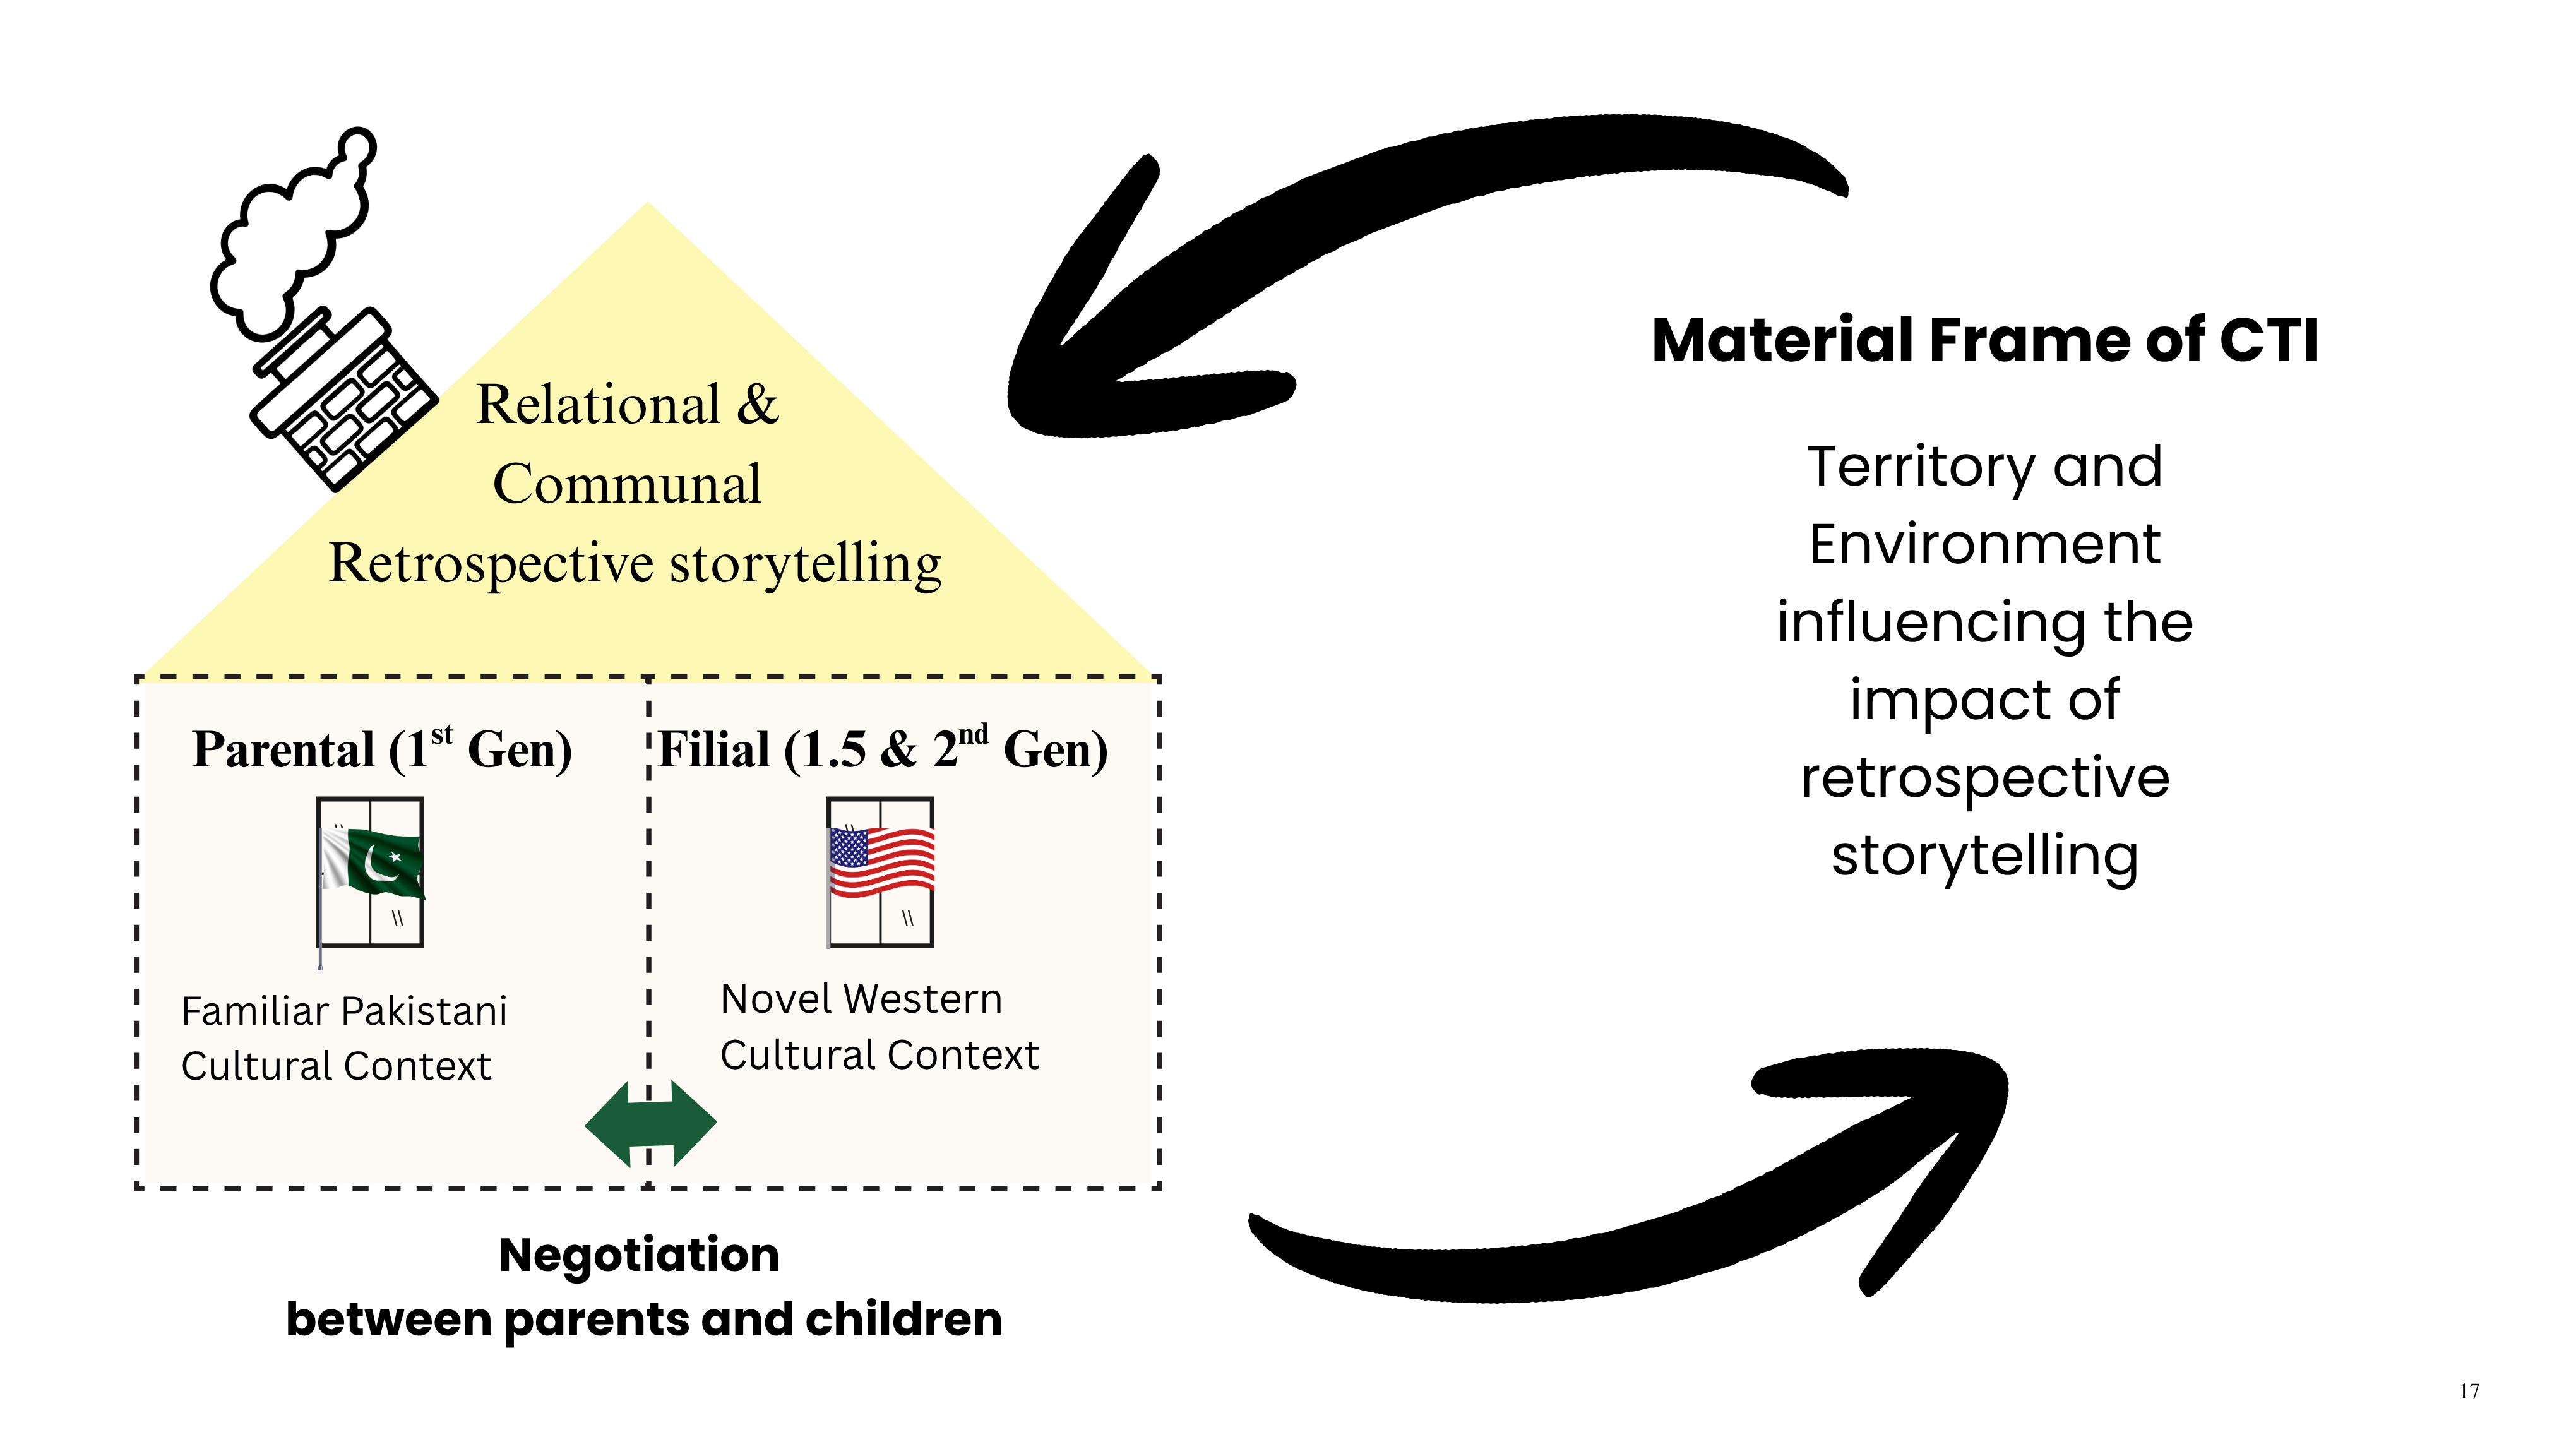
\includegraphics[width=1.00\linewidth]{Dissertation/figures/Final-Model.png}
    \label{fig:final-model}
\end{figure}

This model (see figure 2) therefore proposes that marrying CTI with CNSM’s retrospective storytelling heuristic offers a way to capture how identities are not only individually layered but are also collectively co-constructed through stories that embed cultural values, relational obligations, and personal histories into family decision-making.

The data is collected in the form of narratives of the individual’s lives from a lens of mother or father and children born to migrant parents. The initial data showed the major contribution of relational and communal retrospective storytelling in shaping the decision making of parents towards their children’s life defining decisions, which impact all the layers of their identity. Based on the findings and what data revealed especially in context of the CTI and its five frames and CNSM’s retrospective storytelling heuristics the following model design emerged. 

The dashed (porous) boundary in the model represents the bidirectional flow of influence between parents and children, emphasizing that identity negotiation is not unidirectional. While parents draw heavily on communal and relational retrospective storytelling, children simultaneously bring in perspectives shaped by their engagement with the broader social world such as schools, peers, and institutional environments. These external influences introduce new meanings, values, and identity possibilities into the household, making the negotiation process dynamic and continuously evolving.

Within this space, both parents and children operate with distinct yet interconnected points of view. Parents’ perspectives are largely shaped by communal expectations and diasporic pressures, while children’s perspectives emerge at the intersection of familial narratives and lived experiences within a Western context. The porous boundary thus reflects how these influences move across the household, shaping the magnitude and intensity of identity gaps.

 The findings suggest that communal retrospective storytelling plays a disproportionately stronger role for first-generation immigrant parents. In a context marked by uncertainty and limited familiarity with the host society, parents rely on communal narratives as a primary source of guidance. These stories become a key mechanism for interpreting risks, defining acceptable behavior, and making decisions about their children’s lives. Within this context, communal retrospective storytelling becomes a primary mechanism of sense-making and decision-making. These narratives, often shared as cautionary accounts about children being negatively influenced by Western cultural norms or peer environments, guide parental perceptions of risk and responsibility. Simultaneously, relational storytelling within the family reinforces these narratives, shaping how parents interpret their roles and responsibilities in directing their children’s lives.
 
Importantly, communal retrospective storytelling is also shaped by the material frame of identity, including territorial location, sociopolitical climate, and institutional environments. The material frame influences which stories circulate, how they are interpreted, and how they are enacted. At the same time, it serves as the primary site where identity negotiations become visible, as outcomes are reflected through physical appearance, embodied practices, behavioral norms, and even health and well-being.

Thus, while all CTI layers; personal, enacted, relational, communal, and material operate simultaneously and remain deeply interpenetrated, the material frame does not function independently. Rather, it acts as a reflective lens through which the alignments, tensions, and negotiations across all identity layers are projected into the visible, social world.

As a result, identity negotiation within immigrant households unfolds under the combined influence of relational and communal retrospective storytelling, shaped and constrained by the material environment. The porous nature of this negotiation space highlights that identity gaps are not fixed but are continuously produced, negotiated, and recalibrated through ongoing communication.

 The data highlighted the significant role of relational and communal retrospective storytelling in shaping parental decision-making about children’s early life defining trajectories. These stories, told and retold within families, function as interpretive frameworks through which parents make sense of their own experiences and project values, fears, and aspirations onto their children. Parents’ own self-conceptions as responsible providers or protectors are affirmed in the stories they tell about their sacrifices. Relational retrospective storytelling positions children as extensions of the parents’ identities, responsible for carrying forward family honor, security, and cultural values. Communal retrospective storytelling situates decisions within broader cultural logics that transcend the personal and relational identities. Such decisions when and whom they should marry become sites where identity is negotiated and layered. While the 1.5 generation still gave in mostly and obliged, the second-generation children, men in particular resisted and made their own decisions even if that meant distancing themselves from the parents.
 
Sami knew his father was not in favor of him getting married to now his wife. In order to avoid the any awkwardness or conflict during the festive events, he called his father and told him to not attend his wedding while rest of the family members were the part of the celebrations, which were done in accordance with both partners religions, i.e. Hindu and Muslim wedding ceremony.

 Stories about the past often blur boundaries, demonstrating how one frame (e.g., communal) penetrates another (e.g., personal, or relational identity). Jia’s parents felt unsafe sending their daughters to high school based on communal stories of other men in the building.
 
Children have noticed their parents' deteriorating health as result of immense stress and guilt for not being able to support their elderly parents back home while struggling to adjust to the viewpoints of their growing children in the US. Teenagers and children in their early twenties have a higher level of conflict and confusion regarding getting the validation of parents for their outlook on life. Daughters have mostly reported disapproval of the choices they made by the mothers including going to concerts, prom and other school dances or homecoming. Mostly, the eldest daughter had to take the fight to get permission to attend these events. One participant remembered how she had to fight to go to homecoming game and she was only allowed until half time while her parents sat in the car waiting for her to get back. She recalled how both parents were in a bad mood when she got in the car. Similarly, young men have faced challenges in career choices and finding their life partners and disapproval came more from their fathers. For young men, the expectation of being the provider meant that their career choices were limited to the financially stable ones, and they were discouraged from more creative or uncertain professions. They were also conditioned to be emotionally stoic and not show any vulnerability.

Many parents, suffer physically and emotionally worrying about aging parents back in Pakistan who are often alone and without adequate support. This creates a profound sense of guilt for not being able to be present during their parents’ times of illness, emotional distress, or final moments. That guilt deeply impacts these mothers and is often passed down to their children, who, in turn, struggle with not knowing how best to ease their parents’ pain.

Retrospective storytelling about the struggles families faced back home, particularly witnessing mothers under constant stress, overextending themselves to provide for the family, and prioritizing their children’s education, often instills a deep sense of responsibility in children. This sense of duty motivates them to pursue education and careers that would enable them to support their families and ease their parents’ financial burdens.

The interactions between first-generation and second-generation Pakistani Americans in the US are further shaped by several intersecting factors, including education level, mode of entry into the US, reasons for migration, family background, and the socio-economic status of extended families back home. Additionally, the type of family system whether joint or nuclear, and whether individuals belong to the second generation further influence these intergenerational dynamics and experiences.

\textbf{No, It Hasn't Been Easy}

\begin{FoundPoem}
No.
It hasn't been an easy life, if I look back
especially the years I spent in Cleveland
work full time
take care of two kids.
It was a very tough life.
If I turn around and look back,
I don't know how I did it.

But, by the grace of God,
the time has passed,
I'm ready to die any day
I don't want to have another life

 keep telling my kids that.
my daughter says,
"You used to say that to me when I was 9.
Do you realize how hard and traumatic that was for 9 years old,
 to listen to your mother talking about her death?"
been a very hard life,	
 but,		 by the grace of God,
much better 	than					 so many people.
especially now
people 		a tough time in Gaza,
I see them,	 say		I had a very easy time
compared to them.
\end{FoundPoem}

The stories demonstrated a strong relationship between first-generation peer storytelling and the relational and intergenerational meaning-making of values and beliefs within Pakistani American families. Stories shared among first-generation parents (particularly within community and peer networks) functioned as cautionary narratives that shaped how parents interpreted parenting practices, cultural boundaries, and future outcomes for their children. These narratives intersected with multiple contextual factors, including migration pathways, religious expectations, school environments, and gendered moral judgments. For instance, Zubi’s father’s migration decision was influenced by family pressure and emotional guilt towards the suffering of his mother. In later community stories such as people and peers from the community advising younger children to cover heads and wear hijab reinforced expectations of visible religious ethnic identity. Similarly, Maheen’s father quitting his administrative job in Pakistan to move to the US and work as a cab driver, suggested by his childhood friend who was already settled in that job in Chicago reflects how institutional and social spaces further amplified these narratives. Within the framework of CNSM, storytelling functions as an act of communicating narratives. The content and process of storytelling play an integral role in identity development and making an individual a part of society or community, transmitting cultural meanings, values, and beliefs, facilitating sense-making and coping in the face of adversity, and fostering relational connections \citep{koenigkellasFamilyStoriesStorytelling2012, koenigkellasCommunicatedNarrativeSenseMaking2022}.

Based on my understanding of the theoretical framework of Communicated Narrative Sense-Making (CNSM), the retrospective storytelling heuristic examines how people frame both the stories they tell and the stories they hear, highlighting the significant link between this storytelling process and the development of individual and relational identity, sense-making, and overall well-being \citep[p.~120]{koenigkellasCommunicatedNarrativeSenseMaking2022}. 

For first-generation migrant parents, storytelling and social norms exert both conscious and unconscious influence. These norms are drawn not only from the societies they left behind in Pakistan but also from the Pakistani and Muslim communities they engage with in the environment and territory surrounding them. As \citet[Ch.~5]{perloffDynamicsPersuasionCommunication2023} defines, social norms are “unwritten rules shared by a group or society about how we should behave.” Within this framework, major life decisions that parents make for their children are often shaped by social norms set by communal retrospective storytelling in ethnic religious communities establishing a subculture within the broader diverse society of the US, which reinforces pressures to conform to collective expectations. These narratives act as guiding forces, providing familiar cultural frameworks for parenting and decision-making while simultaneously reducing uncertainty in navigating the unfamiliar US cultural and social expectations as well as the educational system with its broader material environment. As the data showed, parents felt strongly about protecting their children (daughters in particular) from the hyper-sexualized concepts of freedom and teenage romance. The decisions of parents are not just influenced by the factors of communal retrospective storytelling but also based on their lived experiences while growing up in Pakistan. Parenting in the US presents many challenges, and for daughters, the pressures often feel even more complex than for boys. As a 36-year-old mother based in Texas, for example, chose to homeschool her four children until high school. Her decision was shaped by her own experiences of mistrust and lack of support during her school years. She does not want her children to endure the same hardships.

For many immigrant parents, the impulse to protect their children arises from their own experiences of struggle, leading to an inner conflict and confusion. While they seek to shield their children, the processes of identity development and negotiation within Pakistani households are deeply influenced by parents’ own upbringings and the ways their early experiences shaped their sense of self and social standing among peers. These histories, in turn, affect their major life decisions as adults and parents.

\section{Addressing the Research Questions}

Circling back to the individual research questions, the findings reveal that participants’ responses were deeply interconnected, with themes overlapping and coexisting across questions rather than aligning in isolation. As such, the answers to each research question are addressed holistically through these intersecting themes, as outlined below.

\subsection{RQ 1: Retrospective storytelling and narrative sharing to make sense of identities within Pakistani American household and in public}

Findings indicate that retrospective storytelling and narrative sharing function as central, everyday communicative practices through which Pakistani American families make sense of their shifting identities across both private and public contexts. These narratives are not episodic but embedded in daily interactions, serving as a primary means through which identity is interpreted, negotiated, and transmitted across generations.

Within private family spaces, parents particularly mothers more frequently engage in storytelling that traces their life trajectories from Pakistan to the United States. These narratives often center on journeys shaped by kismat (fate), family obligations, and educational aspirations, while also foregrounding the stress and uncertainty associated with immigration policies, legal status maintenance, and early financial hardships. Through such storytelling, parents construct a moral and emotional framework that situates their present lives within broader histories of struggle, resilience, and purpose.

Language plays a critical role in this process. Parents intentionally prioritize teaching Urdu to their children as a means of maintaining cultural continuity and enabling intergenerational communication with grandparents and extended family in Pakistan. At the same time, language shapes the very possibility of storytelling itself; the ability of parents and grandparents to narrate past experiences, and for children to fully comprehend them, is mediated through linguistic access. In this way, language becomes both a bridge and a boundary in the transmission of identity narratives.

In public contexts, parents often seek out community through mosques and Pakistani or broader South Asian networks, creating spaces of familiarity and shared understanding with others navigating similar migration experiences. These spaces function as sites of belonging where cultural practices, language, and values are reaffirmed. However, challenges emerge more prominently in broader social settings beyond these communities. Identity negotiations in such contexts are frequently shaped by visible markers such as skin color, the presence or absence of hijab, and accents, which influence how individuals are perceived and treated.

These dynamics vary across generations. While first-generation immigrants may experience marginalization through language and accent, second- and later-generation individuals often navigate assumptions imposed on them based on physical appearance alone. At times, individuals across different generations are homogenized and positioned similarly within dominant social contexts, with little recognition of their distinct lived experiences, levels of acculturation, or identity negotiations. As a result, retrospective storytelling in public becomes a tool for navigating these misalignments allowing individuals to explain, resist, or reframe externally imposed identities while negotiating their place within both cultural and broader societal structures.
Communal retrospective storytelling at times leads parents to unintentionally dismiss or minimize the struggles their children encounter in public contexts, especially through the early school years. As children navigate pressures to fit into dominant cultural norms while maintaining familial and cultural expectations, their challenges are often overshadowed by parental narratives of sacrifice and resilience. This creates a tension in which children’s lived experiences of identity negotiation are rendered less visible or less legitimate within the family discourse.

Aisha recalls:

\begin{FoundPoem}
    
    When I used to go to school, 			and my mom would make
    me dress in Pakistani clothes, and I'll be like, no, I'm not wearing that to
    school. That's embarrassing. 


    Even on 4th of July my mom would make us wear shalwar kameez. It's an
    American holiday, it would be super embarrassing. I'm gonna be honest like I
    would be embarrassed to wear that and go outside.

\end{FoundPoem}

\subsection{Shifting Identities}

Shifting identities refer to ongoing negotiations, reconstructions, and adaptations that individuals undertake as they make sense of themselves within changing cultural, relational, and material contexts \citep{hechtCommunicationTheoryIdentity2021,shinCommunicationTheoryIdentity2017}. Within Pakistani American migrant families, these shifts emerged as parents and children moved between territories that offered differing interpretations of same identity layers: personal, enacted, relational, communal, and material, responding to evolving expectations, social positions, and lived experiences in both Pakistani and American environments.

Both generations’ identity negotiation is highly influenced by retrospective storytelling; the storytelling not only reflects the individual, relational and intergenerational meaning making, but also the values and beliefs, the trauma, and individual’s hierarchical standing and familial expectations. Overall, the findings illustrate how retrospective storytelling activates multiple layers of identity simultaneously articulating personal histories, enacting identity through communication, positioning family relationships, and reinforcing communal values while also anchoring these meanings within material conditions of immigration.

\subsection{RQ 2 and RQ 3: The content and process of storytelling and the material frame of CTI}

The findings reveal that while all five CTI layers operate simultaneously, the material frame plays a particularly salient role in making identity processes observable. It is through material conditions such as visible markers of difference, institutional environments, and geographic location that participants experience moments of alignment or dissonance across identity layers.

In this study, the material frame emerges as the primary site where identity gaps surface. While personal, relational, and communal identities may coexist in fluid and less visible ways, the material frame renders these dynamics tangible. 

As seen in data, at the individual level, participants interpret their identities through material comparisons between “here” and “back home”, between scarcity and opportunity, and between their own experiences and those of more privileged peers. At the relational level, storytelling becomes a mechanism through which families negotiate expectations, often invoking material sacrifices (stress, poor physical)to justify parental authority and to shape children’s sense of duty and belonging. Intergenerationally, these narratives function as vehicles for transmitting values tied to hard work, endurance, and collective uplift, while simultaneously embedding emotional weight and obligation within everyday material realities.

Importantly, the material frame is not a passive backdrop but an active force in identity construction. The material frame becomes evidence of success or failure of parents in keeping the link of their children to their cultural and religious roots alive. Hence material layers serves as markers of moral worth, reinforcing hierarchies within the family and shaping how individuals understand their place across contexts. 

CTI’s identity layers do not operate in isolation; rather, they are simultaneously in play, overlapping and coexisting in dynamic interaction. Identity is not experienced as discrete components but as an ongoing negotiation across personal, enacted, relational, communal, and material layers that are continuously informing one another. Within this interplay, the material frame becomes particularly significant—not because it functions independently, but because it renders these otherwise fluid negotiations more visible.

The material layer provides a tangible site through which identity gaps, dissonances, and negotiations across layers become perceptible. Through physical appearance, dress, bodily attributes, health, and spatial positioning, individuals embody and perform identities that are shaped by the expectations of specific environments. These visible markers often reveal tensions between internal understandings of self, relational expectations, and communal norms. In this way, the material frame acts as an entry point for observing how individuals adjust, align, or resist identity performances in response to place-based pressures, making the simultaneous operation of all identity layers both observable and analytically traceable.

\subsection{RQ 4: Identity gaps and negotiation among Pakistani immigrants}

Identity gaps within CTI emerge when there is misalignment within or between identity layers such as between personal and enacted, personal and relational, or communal and material identities so on. This study extends CTI by demonstrating that these gaps are not only structural but are actively produced and sustained through retrospective storytelling practices. In particular, the findings identify in theme 5 a phenomenon of generational treadmill of guilt, a cyclical process through which narratives of sacrifice, hardship, and parental struggle are transmitted across generations, shaping identity expectations and constraining identity negotiation. 

RQ 4 investigated the identity gaps and negotiation emerge from tensions both within and across CTI layers and are projected through material frames. These gaps are also not static but are dynamically produced through ongoing interactions between family expectations, communal retrospective storytelling, and broader sociopolitical environments (material frame).

One prominent gap seen is between the personal and relational layers, where 1.5 and 2nd generation (children) sense of self may not align with parental expectations shaped by communal retrospective storytelling. Parents’ reliance on communal narratives often rooted in fear of cultural loss or moral deviation led to restrictive decisions that conflicted with children peer’s lived realities and developmental needs (homeschooling throughout the Highschool). This created tension, as children navigate between honoring familial expectations and asserting their own identities.

Additionally, gaps between the enacted and ascribed identities become visible in public contexts, where individuals are often perceived based on physical markers such as skin color, hijab, or accent. These external ascriptions may flatten generational differences, positioning first- and later-generation individuals similarly despite their distinct experiences. In response, participants engage in strategic identity negotiation through selective disclosure, adaptation, or resistance to manage these misalignments.

Importantly, the material frame makes these identity gaps more visible. Through embodied markers, spatial contexts, and environmental expectations, individuals experience and negotiate tensions across identity layers in tangible ways. These gaps, while often sources of conflict, also function as sites of meaning-making, where individuals actively reconcile competing demands and construct hybrid, context-responsive identities.

\subsection{Summary of Findings and Discussion}

Together, these findings demonstrate that identity negotiation among Pakistani American families is a layered, relational, and materially situated process, where retrospective storytelling both reveals and mediates identity gaps, enabling individuals to navigate the tensions between who they are, who they are expected to be, and how they are perceived across contexts.

Overall findings demonstrated that no two lives are identical, even when individuals share overlapping characteristics, experiences, or physical attributes. At the same time, the analysis revealed overarching shared experiences, emotions, and life events that have left deep and enduring imprints on participants’ lives from which many have not been able to fully recover. One pervasive theme that emerged across generations was guilt intertwined with trauma. While this trauma manifested in different forms and contexts for different individuals, its presence was evident across generational lines.

When left unacknowledged or unhealed, trauma was shown to circulate intergenerationally through retrospective storytelling, shaping emotional regulation, relational dynamics, and physical wellbeing in subsequent generations. First generation participants described an added layer of guilt and distress associated with immigration, particularly during the first two to five years of transition, a period marked by instability, uncertainty, limited travel back and forth to home country, identity disruption, and the struggle to reestablish social, professional, and cultural belonging.

Findings suggest that identity gaps are not incidental but are systematically produced through the intergenerational circulation of retrospective narratives. The “generational treadmill of guilt” emerges as a key mechanism through which these gaps are sustained. Parents’ storytelling, often centered on sacrifice, immigration hardship, and moral responsibility, constructs a relational framework in which children’s identities are expected to align with these narratives. As a result, second-generation participants frequently navigate tensions between their personal identities and the relational and communal expectations imposed upon them. These tensions are further intensified within material contexts, such as schools, peer group and social environments, and workplaces, where competing norms require alternative identity performances. Thus, identity negotiation becomes an ongoing process of reconciling these gaps, with individuals employing strategies such as adaptation, selective disclosure, resistance, or hybrid identity construction.

Before any upward socioeconomic mobility occurs, many immigrant families experience a steep downward trajectory, characterized by professional loss, financial strain, social isolation, and identity dislocation. The health and wellbeing of first-generation immigrants were found to bear the heaviest burden during this period. For some, distress surfaced through unrecognized or undiagnosed symptoms, while others experienced a wide range of chronic and acute health conditions, including cardiac events, diabetes, autoimmune disorders, anxiety, gastroesophageal reflux disease (GERD), and migraines. These findings underscored how migration-related stressors are not only emotionally taxing but also materially and bodily lived, leaving lasting consequences for individuals and families.

Importantly, storytelling was not unidirectional. Information sharing also emerged through children’s questions, prompted by their observations of family interactions and unfolding events as they grew older. In Aisha’s case, her lived experiences within the household validated and gave material form to the stories shared by her mother, reinforcing their emotional truth and shaping Aisha’s understanding of family history, relational dynamics, and her own identity.

Overall, this dissertation conceptualizes identity as negotiated, materially constrained, and narratively governed across generations. Communal retrospective storytelling functions as shared decision-making infrastructure through which immigrant families collectively interpret past experiences of Pakistani community members in their surroundings to manage present uncertainty and anticipate future outcomes of their children. This framework highlights how identity is continuously produced through the interplay of material conditions, relational and communal retrospective storytelling, and relational negotiation within immigrant family systems.

The collective monologue, the unheard composite voices of children (1.5 and second generation) shaped into a single lived dialogue of immigrant childhood and young adulthood.

\begin{FoundPoem}
We grew up in here (US) and there (Pakistan),
 small towns, villages or big cities
 family homes where everyone belonged to everyone.
 
Some of us were twins.
Some of us were the eldest.
Some of us were raised by grandmothers and aunts
because our mothers couldn’t carry all of us at once.

We called Nani our mother
before we learned the truth.
When our real mothers cried quietly,
we didn’t know why.

They couldn’t visit their parents
 for years at times over a decade.
 
We lived as families 
 first in a studio,
 then in a one-bedroom apartment, or in huge houses
 
We struggled.
But we were told others back home struggled more.

Even when we had little here,
we were reminded that to them
we had everything.

Our mothers worried
They worried for everyone except themselves.

People always had something to say.
You gained weight, skin color is getting darker.
Your sister is prettier or smarter

Our fathers had degrees.
Our mothers were educated

Here (US), they drove cabs.
Worked at gas stations.
The community tried to help,
but their world stopped at gas stations and cabs.

If we had been older,
 we would have said,
 Try an office job.
 Anything.
 
But we were children.

We learned early to go with the flow.
To be okay with whatever happens.

We learned not to say no.
Not to question.
Not to talk about feelings.

This happened.
 We’re NOT going to talk about it.
 Tomorrow is a new day, new start.

So we let it go
 into our bodies.
 
To numb what we didn’t know how to name.

We struggle with sharing emotions.
 Understanding ourselves and them.
 Communicating with them.
 
When emotions get big,
 we black out.
 We can’t remember how we felt.
 
Our defense is blocking it out
and focusing on whatever positives remain.

Some of us turned to prayer.
Kneeling on the jainamaz.
Surrendering to God.

We were told no medication or therapy, can heal 
what just faith, can.

We are working mothers, students, caretakers, sons and daughters.

We are American in our lives and Pakistani in our obligations.

We do our best to cater to their world
 without letting it hold us back.
We love them.
We respect them.
We carry their sacrifices.

And we are still learning
 how to carry ourselves.    
\end{FoundPoem}

Below is the collective Voice of Parents shaped into a single lived monologue for their children.

\begin{FoundPoem}
Dear Beta,
You grew up in between.
We know that now.
 At home you were one thing.
 Outside, felt  another.
 You learned early how to read a room,
how to explain yourself, how to carry an identity that others questioned.
We saw you ask, why do I look different? Why do I sound different?
We wish we could answer your questions better or knew how to help.
We didn’t.


What we want you to know is this: You were never meant to shrink to fit anyone’s comfort.
We did not raise you to live our lives.
We raised you to live yours.

If we held back, it was fear,

Not control.
If we stayed silent, it was survival, not indifference.
If we said “there is a time and place,”
it was because we were taught that love and restraint lived together.

We are still learning.

Believe what grounds you.
Practice faith with intention, not fear.

You are not abandoning us by becoming yourselves.
You are continuing us in ways we could not imagine
\end{FoundPoem}